\chapter{Experimentación}


\section{Introducción}

En el capítulo~\ref{chap:metricas} se han mencionado un conjunto de métricas individuales objetivas que se enfocan en destacar alguna característica específica de un algoritmo (por ejemplo da mayor ponderación a los errores que se encuentran en el rango intermedio de un objeto de referencia por el impacto en el reconocimiento de formas) y que en su conjunto dan una idea global de desempeño de un algoritmo. En general la comunidad de investigación ha propuesto diversos y variados métodos para evaluar los algoritmos que utiliza este proyecto, presentando muchas veces sus resultados en una de estas métricas. El propósito de este capítulo es revisar estas métricas y verificar las más adecuadas para este proyecto. 

Para evaluación de desempeño se han utilizado dos enfoques complementarios; medición a nivel de píxel, basado obtener las tasa de falsas alarmas (falsos objetos detectados) y fallas de detección (zonas que no son detectadas) para construir la curva de operaciones características (ROC), descritas en la sección \ref{subsec:roc} del capítulo \ref{chap:metricas} y mediciones a nivel de cuadro (imágenes), las cuales son métricas que miden similaridad (\textit{PSNR}, \textit{SSIM}, \textit{D-SCORE}) o correlación (\textit{MCC}, \textit{F-Measure}) entre la imagen (mascara) resultante y su referencia (\textit{ground-truth}). La combinación de ambos enfoques, proporcionan un rendimiento global de los algoritmos evaluados en cada una de las secuencias del conjunto de datos MuHAVI \cite{singh_muhavi_2010}.



\section{Conjunto de datos de acciones humanas - MuHAVI}



El conjunto de datos MuHAVI\cite{singh_muhavi_2010} (\textit{Multicamera Human Action Video}), es un repositorio de secuencias de video con 17 clases diferentes de acciones humanas, tomadas desde distintos ángulos de observación (ver descripción en tabla \ref{tab:acciones}).  Las acciones son realizadas sobre un escenario rectangular, iluminado con un tipo de focos empleados en vías públicas para alumbrado nocturno. Las diferentes acciones son registradas por 8 cámaras dispuestas en las cuatro esquinas y costados de este escenario rectangular, como se indica en los ejemplos de la figura \ref{fig:muhavi_cameras}. El tipo de cámaras e iluminación, así como la distancia de las cámaras a los actores, y las irregularidades del escenario, simula un típico escenario de vigilancia nocturna de circuito cerrado por televisión (CCTV) y son parte de los desafíos que deben abordar los algoritmos de pruebas, al usar MuHAVI como datos de experimentación.

Este conjunto de datos fue desarrollado para satisfacer varios propósitos: evaluación de métodos de reconocimiento de acciones humanas basados en siluetas (\textit{silhouette-based human action recognition} - SBHAR), que pueden hacer uso del conjunto de imágenes anotadas manualmente como medio de comparación de resultados, evaluación de segmentación contrastando resultados de algoritmos con las imágenes \textit{ground-truth} que dispone este conjunto de datos, suministrar un conjunto de pruebas en investigaciones orientadas a la construcción de imágenes 3D, debido a sus imágenes similares desde diferentes ángulos o vistas.

\begin{figure}
\centering     %%% not \center
\subfigure[Vista de las 8 cámaras sobre el escenario con diferentes ejemplos de acciones]
{\label{fig:MuHAVI_Cameras}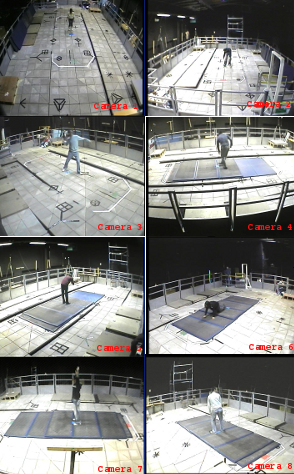
\includegraphics[width=60mm]{img/ch6/MuHAVI_Cameras}}
\subfigure[Disposición de las 8 cámaras sobre el escenario]{\label{fig:MuHAVI_Cameras_Stage}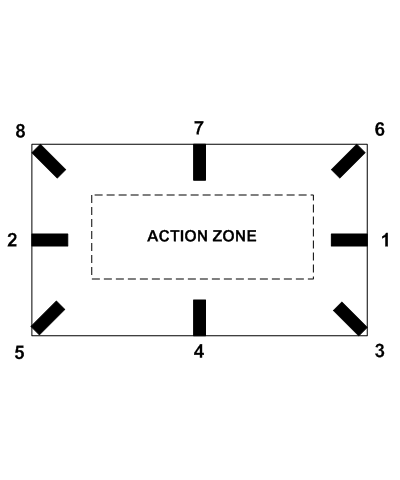
\includegraphics[width=60mm]{img/ch6/MuHAVI_Cameras_Stage_1}}
\caption[Disposición de las 8 cámaras sobre el escenario]{Esquema general con disposición de las 8 cámaras en el escenario. }
\label{fig:muhavi_cameras}
\end{figure}


 Cada una de las acciones descritas en la tabla \ref{tab:acciones} fueron desarrolladas por 14 actores, y cada actor ejecuta 3 veces una determinada acción, resultando un total de 8x17x14=1904 de segmentos de video. Sin embargo, sólo se encuentran disponibles para la comunidad 8x17x7=952 segmentos de video (las acciones realizadas por 7 actores), en secuencias de imágenes JPEG. Dentro del total de videos que proporciona MuHAVI, existe un subconjunto secuencias con imágenes de referencia o \textit{ground-truth} (imágenes segmentadas correctamente), que permite evaluar el rendimiento de los algoritmos a nivel de píxel . Esto es, detectar todos los píxeles activos dentro de una imagen y luego contrastar con los píxeles de su imagen de referencia. Este subconjunto está compuesto por las cinco primeras clases indicadas en la tabla \ref{tab:acciones} (\textit{WalkTurnBack}, \textit{RunStop}, \textit{Punch}, \textit{Kick}, y \textit{ShotGunCollapse}), ejecutadas por dos actores (denominados \textit{Person1} y \textit{Person4}), desde las cámaras 3 y 4, obteniendo un total de  5 x 2 x 2=20 acciones. Las acciones realizadas por el actor denominado \textit{Person1}, de cada una de las secuencias, contiene un gran número imágenes previas a la acción que va ser ejecutada, esto garantiza, en caso de ser necesario, el tiempo necesario para que los algoritmos puedan estimar el modelo del fondo de imagen.

\begin{table}
\centering
\scalebox{0.8}{
\begin{tabular}{ c | c  }
\hline
ACTION CLASS & ACTION NAME \\ \hline
C1 & \textbf{WalkTurnBack} \\ \hline
C2 & \textbf{RunStop} \\ \hline
C3 & \textbf{Punch} \\ \hline
C4 & \textbf{Kick} \\ \hline
C5 & \textbf{ShotGunCollapse} \\ \hline
C6 & PullHeavyObject \\ \hline
C7 & PickupThrowObject \\ \hline
C8 & WalkFall \\ \hline
C9 & LookInCar \\ \hline
C10 & CrawlOnKnees \\ \hline
C11 & WaveArms \\ \hline
C12 & DrawGraffiti \\ \hline
C13 & JumpOverFence \\ \hline
C14 & DrunkWalk \\ \hline
C15 & ClimbLadder \\ \hline
C16 & SmashObject \\ \hline
C17 & JumpOverGap \\ \hline
\hline
\end{tabular}
}
\caption[Tabla de acciones humanas definidas en MuHAVI]{Tabla que describe el total de acciones humanas contenidas en MuHAVI}
\label{tab:acciones}
\end{table}

\begin{figure}[!ht]
\centering     %%% not \center
\subfigure[Kick]%
{\label{fig:Kick}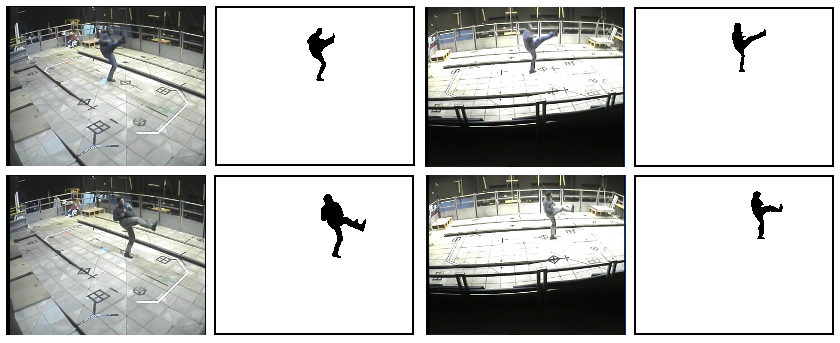
\includegraphics[width=80mm]{img/ch6/Kick}}
\subfigure[Punch]
{\label{fig:Punch}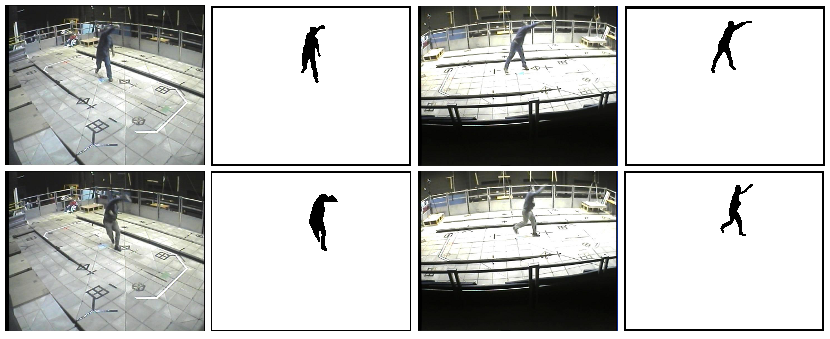
\includegraphics[width=80mm]{img/ch6/Punch}}
\subfigure[RunStop]
{\label{fig:RunStop}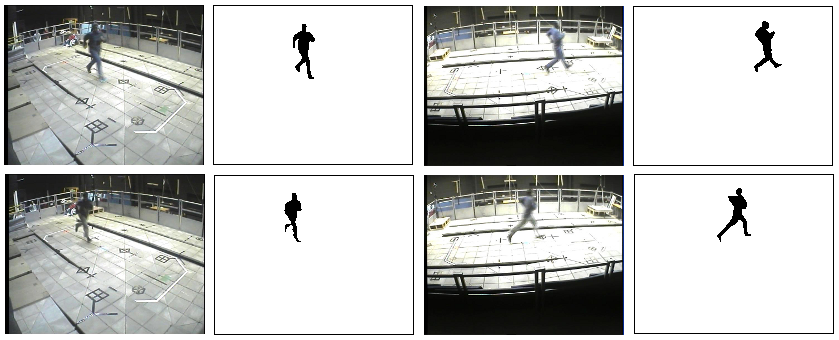
\includegraphics[width=80mm]{img/ch6/RunStop}}
\subfigure[ShotGunCollapse]
{\label{fig:ShotGunCollapse}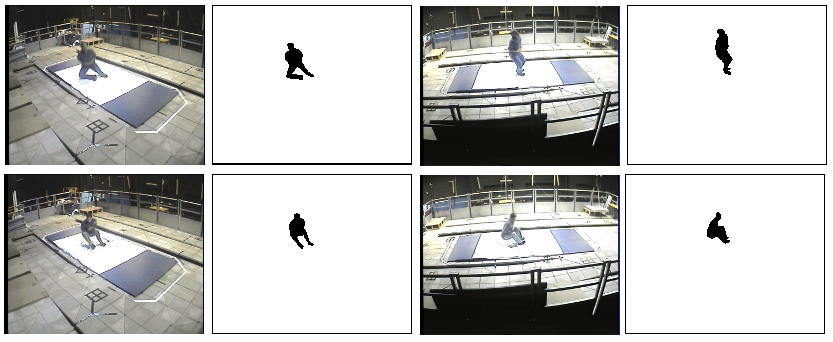
\includegraphics[width=80mm]{img/ch6/ShotGunCollapse}}
\subfigure[WalkTurnBack]
{\label{fig:WalkTurnBack}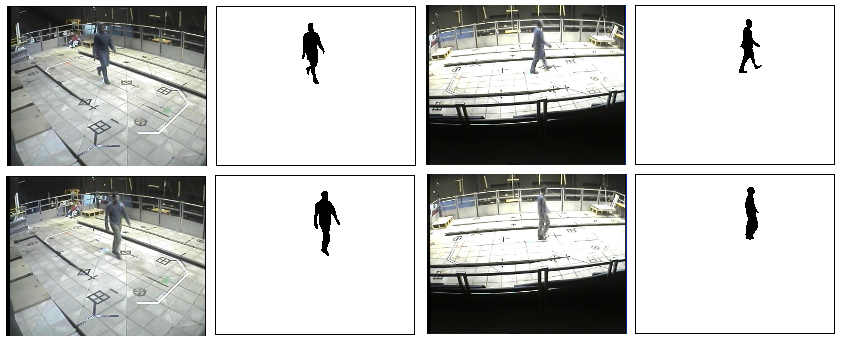
\includegraphics[width=80mm]{img/ch6/WalkTurnBack}}
\caption[Ejemplo de acciones humanas con imágenes de referencias]{Ejemplo de acciones humanas desde diferentes vistas del escenario junto con sus respectivas imágenes de referencia (\textit{ground-truth})}
\label{fig:reference_action}
\end{figure}



\section{Procedimiento de Evaluación}
La evaluación de los algoritmos se basa principalmente en la comparación de sus curvas de operaciones características (\autoref{subsec:roc}), obtenidas mediante la realización de extensos experimentos. De manera visual se puede determinar el algoritmo con mejor desempeño, localizando la curva más cercana al borde superior izquierdo de la gráfica, es decir la curva ubicada sobre las demás gráficas resultantes. Un mejor desempeño se asocia con la curva que presenta una mayor área, con respecto a las otras en un rango específico de evaluación dentro del gráfico. Una mayor exactitud de evaluación se obtiene fijando una tasa de falsos negativos, y luego comparando los valores de verdaderos positivos para el punto de operación determinado, el algoritmo con mejor desempeño es aquel con una tasa mayor de verdaderos positivos con respecto a todos los demás.

Los parámetros más relevantes, para el funcionamiento de los distintos algoritmos descritos en el \autoref{chap:algoritmos}, son el factor de aprendizaje (\textit{Learning Rate}) y el umbral (\textit{Threshold}) que determina la pertenencia de un píxel a la imagen de fondo, o al actor en movimiento. En el caso del algoritmo no-paramétrico (descrito en la sección \ref{sec:modelo_noparametrico}), $\alpha$ es un parámetro del color recomendado en $0.3$ y \textit{Threshold} es la probabilidad que un píxel sea \textit{foreground}. Para el desarrollo de las pruebas se escogieron dos valores de factor de aprendizaje, $\alpha=0.001$ y $\alpha=0.0002$ (tabla \ref{tab:frames}) y se establecieron 21 valores de umbral en un rango de 1 a 100, Los primeros números de este conjunto tiene intervalos de separación 0.5 y 2, los cuales tienen como finalidad agregar más detalles en la parte superior de la curva. 

La construcción de una curva ROC para cada uno de los algoritmo, se consigue manteniendo fijo uno de estos parámetros de configuración (\textit{Learning Rate}) durante la ejecución de todas las secuencias de experimentación, y variando consecutivamente el segundo parámetro (\textit{threshold}) dentro de un rango de valores previamente establecidos. De esta forma, una curva de operaciones correspondiente a una secuencia completa de experimentación, consiste de un conjunto de experimentos delimitados por el par ordenado $\langle\textit{learning rate},\textit{threshold}\rangle$. La salida del procesamiento de un algoritmo, resulta en un punto dentro de la curva de operaciones características, determinados por los valores promedios de TPR y FPR (tasa de verdadero y falsos positivos respectivamente). Finalmente la curva de operaciones es un conjunto de puntos en la gráfica que son producto de la ejecución independiente de un algoritmo por cada par ordenado de estos parámetros. 

El procedimiento de evaluación se realiza sólo con las secuencias de videos que contiene imágenes de referencia, éstas son las clases de acciones C1 a C5 señaladas en la tabla \ref{tab:acciones}. Un punto TPR, FPR en la curva global de operaciones de un algoritmo consiste, como se indica en el párrafo anterior, de una serie de ejecuciones sobre estas secuencias. El resultado global es un promedio de las ejecuciones del mismo algoritmo sobre las 20 secuencias de la tabla \ref{tab:acciones}. La salida del procesamiento de una secuencia (por ejemplo \textit{WalkTurnBack Person1 Camera\_3}) entrega un valor promedio de tasa de verdadero y falsos positivos, éste resultado posteriormente se promedia con las salidas procesadas de las otras secuencias, produciendo un valor global de TPR y FPR para el algoritmo en evaluación con la pareja de parámetros (\textit{learning rate} y \textit{threshold}) seleccionados para el procedimiento de evaluación en particular. De este modo, la construcción de una curva global de operaciones para el total secuencias de vídeo, con dos actores (\textit{Person1, Person2}), adquiridas por dos cámaras (\textit{Camera3 y Camera4}), un valor de factor de aprendizaje ($0.001$ ó $0.0002$), y 21 valores seleccionados para el umbral, requiere $5x2x2x1x21=420$ ejecuciones de un mismo algoritmo. Considerando que el algoritmo que menos demora en procesar el total de las secuencias es cerca de 9 minutos comparado con otro que demora 25 minutos, se tiene un procesamiento total de 3 horas y 9 horas respectivamente.




\begin{table}
\centering
\begin{tabular}{ c | c  }
\hline
$\alpha$ & FRAMES \\ \hline
0.0001 & 1054 \\ \hline
\textbf{0.0002} & \textbf{527} \\ \hline
0.0003 & 351 \\ \hline
0.0004 & 263 \\ \hline
0.0005 & 211 \\ \hline
\textbf{0.001} & \textbf{105} \\ \hline
0.002 & 53 \\ \hline
0.003 & 35 \\ \hline
0.004 & 26 \\ \hline
0.005 & 21 \\ \hline
\hline
\end{tabular}
\caption[Tabla que relaciona el valor de $\alpha$ y número de frames necesarios para que un objeto se mantenga estático.]{Tabla que relaciona el valor de $\alpha$ y número de frames necesarios para que un objeto se mantenga estático.}
\label{tab:frames}
\end{table}



\section{Evaluación de Rendimiento}

La figura \ref{fig:resultado_roc} ilustra las curvas de operaciones obtenidas durante el desarrollo de la experimentación, estas reflejan los resultados conseguidos con dos factores de aprendizaje propuestos para los ensayos ($0.001$ y $0.0002$). La tasa de aprendizaje $\alpha=0.001$, de acuerdo con la tabla \ref{tab:frames}, considera aproximadamente unos 100 cuadros antes que un objeto móvil detenido sea estimado como imagen de fondo, y 500 cuadros para $\alpha=0.0002$. Las curvas incluidas en los gráfico constituyen una combinación global promedio del procesamiento de las 20 secuencias (5 secuencias de acciones humanas, dos actores, y dos cámaras) descritas en la tabla \ref{tab:acciones}, para cada algoritmo en evaluación. Se incorpora también dos gráficos adicionales, con resultados de experimentación utilizando morfología; éste aplica un filtro de erosión que elimina cualquier conjunto de menos de 4 pixeles conectados. Una descripción más detallada con resultados desagregados por acciones, por cámara, y actores se encuentra en Apéndice~\ref{chap:Apendice_2}.

Las curvas logradas en la experimentación están sobre la linea recta $x=y$, de estimación aleatoria (sección \ref{subsec:roc}), dentro del rango de valores $[0-1]$ en el eje de las ordenadas (verdaderos positivos) y $0-0.5$ para el eje de las abscisas (falsos positivos). La forma de las curvas, en todos los diagramas de la figura \ref{fig:resultado_roc}, sigue un patrón que relaciona el comportamiento de ambas métricas en forma directa; se observa que en la medida que el valor de una métrica cambia (aumenta o disminuye) en una dirección de su eje, la otra también cambia en el mismo sentido, pero no en la misma proporción. El incremento (o disminución) en los valores de ambas tasas se consigue modificando en forma discreta los niveles \textit{threshold}. En el caso de los algoritmos basado en mixtura de Gaussianas (\textit{SAGMM}, \textit{MOG2}, \textit{UCV} \textit{Linear} y \textit{Staircase}) incrementos en este valor causan disminución de la tasa de verdaderos y falsos positivos. Pero, en el caso del algoritmo No-Paramétrico incremento en el \textit{threshold} produce aumento en ambas tasas. Se debe recordar, que la tasa de verdaderos positivos (ver sección \ref{subsec:roc}), para la evaluación de reconocimiento de siluetas, es una medida que indica la proporción de pixeles correctamente seleccionados en la silueta, y la tasa de falsos positivos (falsas alarmas) indica una proporción de pixeles de \textit{background} seleccionados incorrectamente como pixeles perteneciente a la silueta. 

En general el algoritmo SAGMM \cite{chen_vehicle_2012} presenta un desempeño promedio mejor con respecto a los algoritmos basado en mixtura de componentes Gaussianas, esto debido que la curva de operaciones se encuentra localizada más cerca del borde superior izquierdo de la gráfica, sobre las otras curvas. Sin embargo la curva del algoritmo No-Paramétrico \cite{elgammal_nonparametricmodel_2000} la sigue de cerca al estar levemente debajo de la curva SAGMM, el cual puede ser interpretado como un rendimiento similar entre ambos algoritmos. El siguiente algoritmo en esta clasificación general de desempeño, se encuentra MOG2 \cite{zivkovic_efficient_2006} y la versión \textit{Linear} del algoritmo UCV \cite{salvadori_gaussian_2012}. Se puede advertir que el algoritmo UCV modelo \textit{staircase} \cite{salvadori_gaussian_2012} mejora su desempeño al sobrepasar la curva UCV \textit{Linear} y luego la de MOG2, entre el rango del 2\% y 6\% de la tasa de falsos positivos, pero sólo con la tasa de aprendizaje $\alpha=0.001$ y su desempeño es inferior al utilizar un factor de aprendizaje de $0.0002$ con o sin morfología. Esta evaluación cualitativa también se ratifica comparando el área bajo la curva, entre el rango $[0-0.15]$ del eje falsos positivos y $[0.4-1.0]$ en el eje verdaderos positivos (indicado en la tabla \ref{tab:auc}) con un valor $\alpha=0.001$. SAGMM tiene un área mayor ($0.12278$) que los otros algoritmos, continua el No-Paramétrico ($0.11771$), MOG2 ($0.09908$), UCV en su versión \textit{Staircase} ($0.09083$), y finalmente \textit{Linear} ($0.08310$).

\begin{table}[!ht]
\centering
\begin{tabular}{ l | c  | c | c}
\hline
Algoritmo & $\Delta X$ & $\Delta Y$ & Área \\ \hline 
sagmm & $0.15-0.001$ & $0.89-0.40$ & \textbf{0.123} \\
np & $0.15-0.007$ & $0.89-0.63$ & 0.113 \\ 
mog2 & $0.15-0.002$ & $0.75-0.40$ & 0.099 \\
ucv\_staircase & $0.15-0.019$ & $0.80-0.40$ & 0.090 \\
ucv\_linear & $0.15-0.016$ & $0.72-0.40$ & 0.083 \\ \hline
\hline
\end{tabular}
\caption[Área bajo la curva de los algoritmos]{Área bajo la curva de operaciones de cada algoritmo.}
\label{tab:auc}
\end{table}

El resultado con $\alpha=0.0002$, figura \ref{fig:plot15-2_1}, modifica ligeramente la localización de la curva SAGMM con respecto a la figura \ref{fig:plot15-1_1} y continúa, junto con el algoritmo NP, presentando mejor desempeño en relación a los demás. Mejora también el rendimiento de los algoritmos MOG2 y UCV \textit{Linear} al producirse un desplazamiento de ambas curvas por encima de su localización anterior. Pero, la versión UCV \textit{Staircase} deteriora notablemente su desempeño, al producir un desplazamiento de su curva hacia el lado derecho; disminuye la tasa de verdaderos positivos y aumenta la tasa de falsos positivos. La mayor influencia del aumento de la tasa de aprendizaje ($\alpha=0.0002$) se manifiesta en los algoritmos SAGMM y MOG2, al aumentar los valores de \textit{threshold} para alcanzar la misma tasa de falsos positivos (notar linea roja en $0.03$). Un aumento en el \textit{threshold} incide en una mejora de las medidas de rendimiento como MCC, FMeasure, y DScore (\ref{sub:metricas_percepcion}). 

Un fenómeno diferente se produce al utilizar el operador morfológico de `erosión' (Capítulo 9 de \cite{digital_image_processing_gonzalez}), en las figuras \ref{fig:plot15-1_2} y \ref{fig:plot15-2_2} se aprecia un efecto de compresión hacia el lado izquierdo de las gráficas, es decir, la tasa de falsos positivos disminuyen y en una proporción menor la tasa de verdaderos positivos. Particularmente los algoritmos UCV deterioran su desempeño, la versión \textit{Linear} por ejemplo no logra sobrepasar el 60\% en la tasa de verdaderos positivos, y la versión \textit{Staircase} no supera el el 76\%, con ambos factores de aprendizaje. El filtro morfológico elimina falsos positivos y negativos (ver \ref{fig:metricas_calidad_estatica}), pero, también en menor medida reduce positivos (pixeles de una silueta), principalmente en las zonas de borde entre la silueta y la imagen de fondo, lo que explica las disminución de la tasa de falsos positivos en todas las curvas.



\begin{figure}[!ht]
\centering     %%% not \center
\subfigure[$\alpha=0.001$]
{\label{fig:plot15-1_1}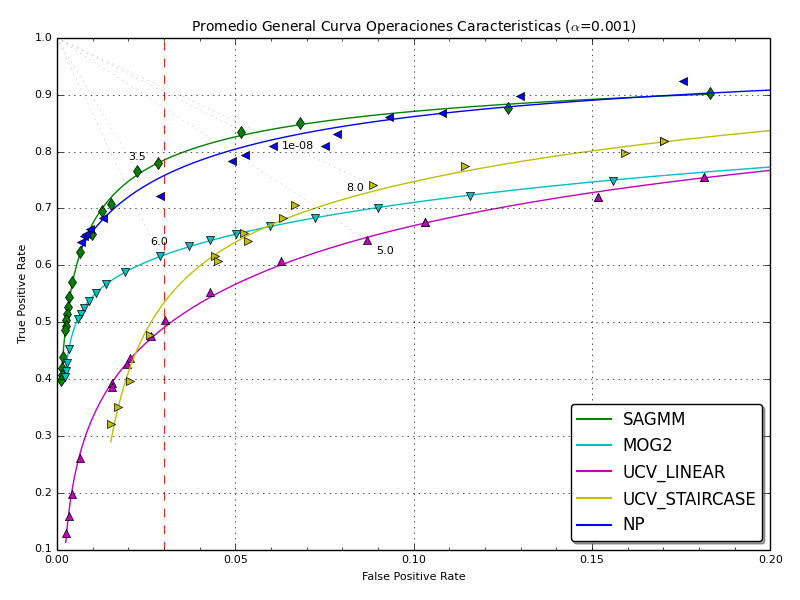
\includegraphics[width=80mm]{img/ch6/plot15-1_1}}
\subfigure[$\alpha=0.0002$]
{\label{fig:plot15-2_1}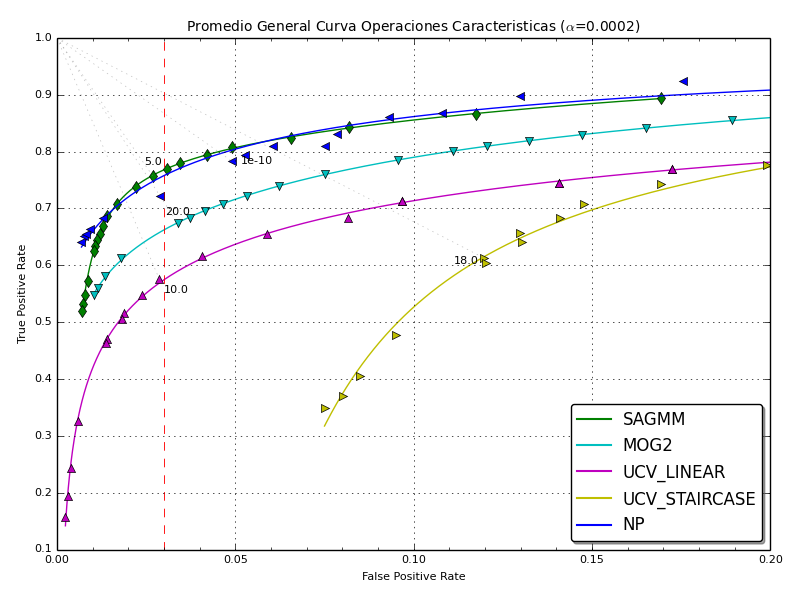
\includegraphics[width=80mm]{img/ch6/plot15-2_1}}
\subfigure[Filtro Morfológico $\alpha=0.001$]
{\label{fig:plot15-1_2}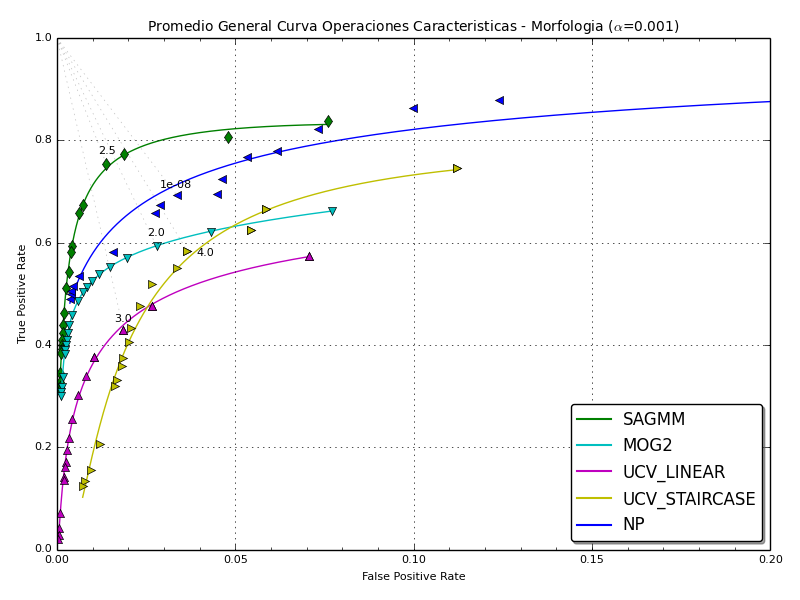
\includegraphics[width=80mm]{img/ch6/plot15-1_2}}
\subfigure[Filtro Morfológico $\alpha=0.0002$]
{\label{fig:plot15-2_2}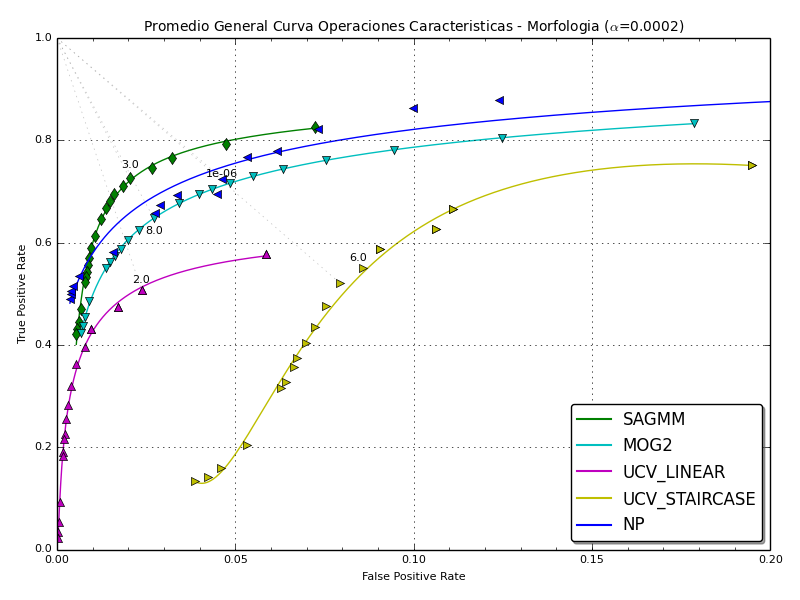
\includegraphics[width=80mm]{img/ch6/plot15-2_2}}
\caption[Curvas de operaciones características obtenidas durante experimentación, usando dos valores diferentes de factor de aprendizaje]{Curvas de operaciones características para dos valores diferentes de factor de aprendizaje de cada algoritmo. En ambas gráficas se ha dejado constante el valor de aprendizaje ($\alpha=0.001$ y $\alpha=0.0002$ respectivamente) y modificado el valor de umbral (distancia de Mahalanobis). Incrementos en el valor de umbral resulta en una disminución constante de la tasa de verdaderos y falsos positivos. Las imágenes inferiores corresponden a experimentos similares con los mismos valores de $\alpha$, aplicando morfología a las imágenes resultantes.}
\label{fig:resultado_roc}
\end{figure}

%----------------------
\subsection{Comparación puntos de operación}

El criterio usado para seleccionar el punto de operación de un algoritmo en su curva de operaciones, consiste en escoger el lugar de la curva más cercano al punto de clasificación perfecta ($0,1$), ver linea segmentada gris en figura \ref{fig:resultado_roc}, este es el punto de mejor compromiso entre la tasa de verdadero y falso positivos. Las tablas \ref{tab:metricas_1}, \ref{tab:metricas_2}, \ref{tab:metricas_3}, y \ref{tab:metricas_4} reporta valores de métricas de rendimiento y desempeño de los puntos de operaciones escogidos de cada algoritmo, para los dos factores de aprendizaje estudiados con y sin morfología. Las métricas registradas en estas tablas se recopilan en las imágenes de la figura \ref{fig:roc_point}.  La variación general de todas estas métricas de rendimiento (\textit{MCC-Matthew’s Correlation Coefficient}, \textit{F-Measure}, \textit{D-Score}, \textit{PSNR}, y \textit{MSSIM}) con respecto a diferentes valores de \textit{threshold} (distancia de Mahalanobis) se muestran en las figuras \ref{fig:pe_metricas_1} y \ref{fig:pe_metricas_2}

\begin{figure}[!ht]
\centering     %%% not \center
\subfigure[Coeficiente Correlación MCC]
{\label{fig:MCC_plot18}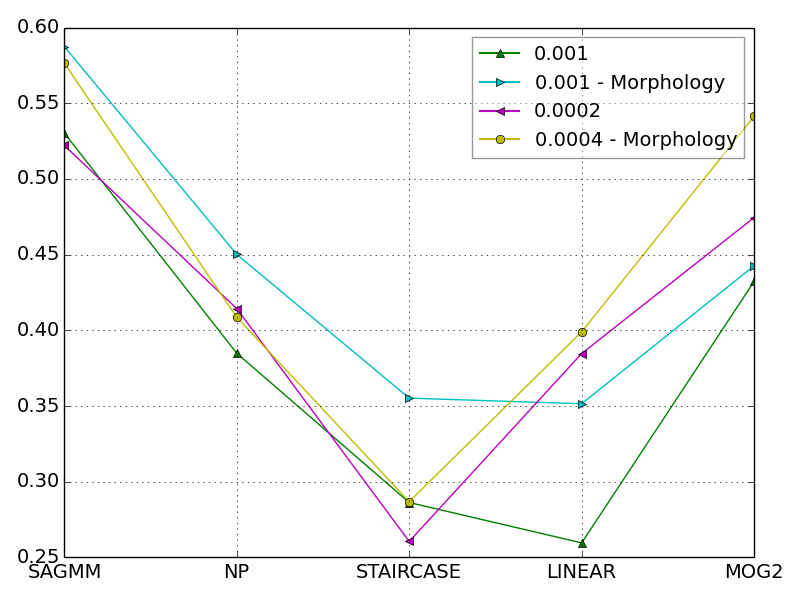
\includegraphics[width=55mm]{img/ch6/MCC_plot18}}
\subfigure[F-Measure]
{\label{fig:FMeasure_plot18}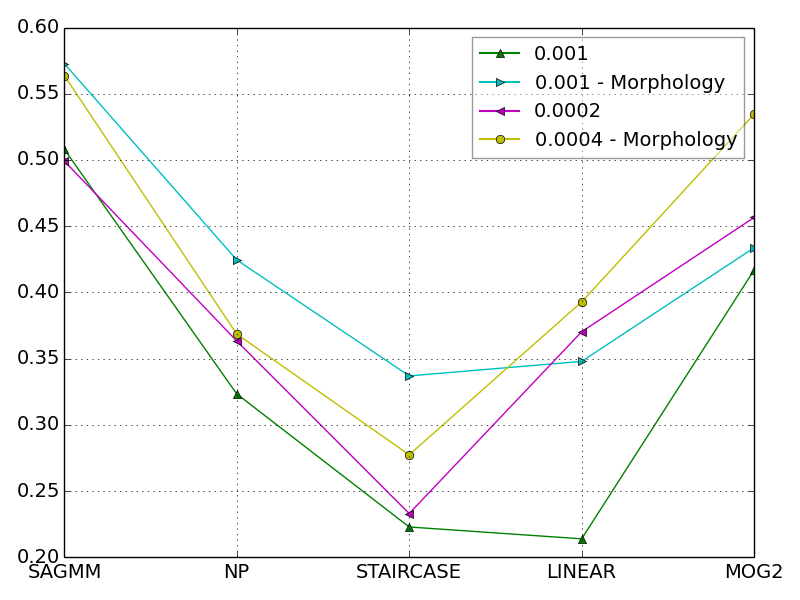
\includegraphics[width=55mm]{img/ch6/FMeasure_plot18}}
\subfigure[D-Score]
{\label{fig:DScore_plot18}\includegraphics[width=55mm]{img/ch6/DScore_plot18}}
\subfigure[Similitud estructural - MSSIM]
{\label{fig:MSSIM_plot18}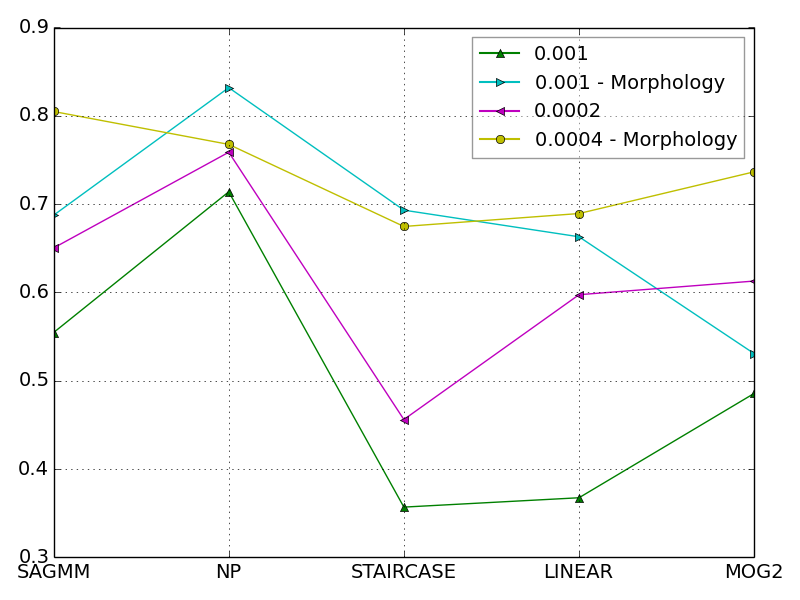
\includegraphics[width=55mm]{img/ch6/MSSIM_plot18}}
\subfigure[PSNR]
{\label{fig:PSNR_plot18}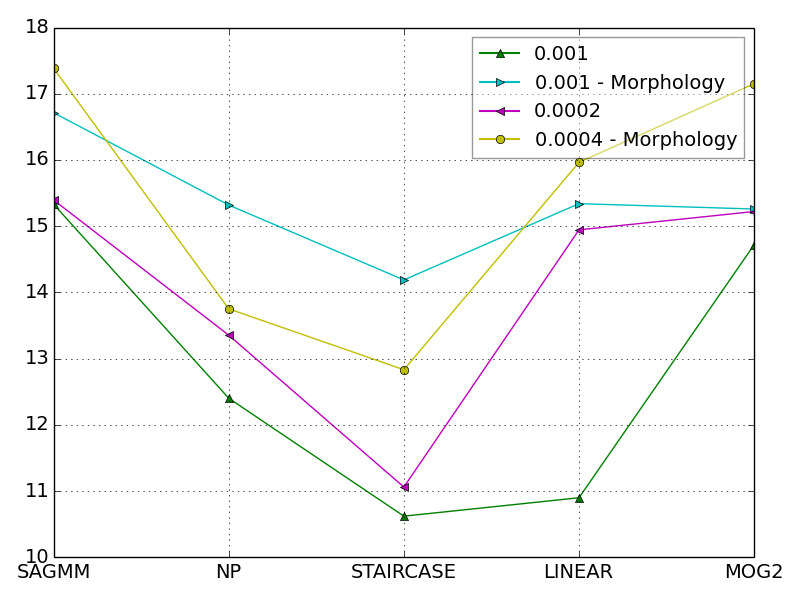
\includegraphics[width=55mm]{img/ch6/PSNR_plot18}}
\caption[Mediciones de rendimiento global obtenidos para un factor de aprendizaje $\alpha=0.001$]{Comparación de métricas de calidad de los puntos de operación escogidos señalados en las tablas \ref{tab:metricas_1}, \ref{tab:metricas_2}, \ref{tab:metricas_3}, y \ref{tab:metricas_4}}
\label{fig:roc_point}
\end{figure}



%\begin{figure}[!ht]
%\centering     %%% not \center
%\subfigure[MCC ($\alpha=0.001$)]%
%{\label{fig:MCC-plot9-1}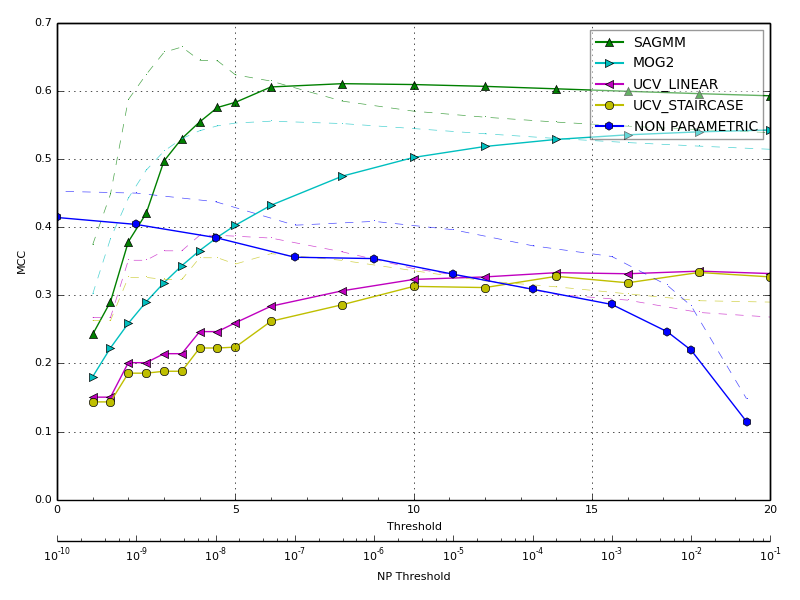
\includegraphics[width=80mm]{img/ch6/MCC-plot9-1}}
%\subfigure[MCC ($\alpha=0.0002$)]%
%{\label{fig:MCC-plot9-2}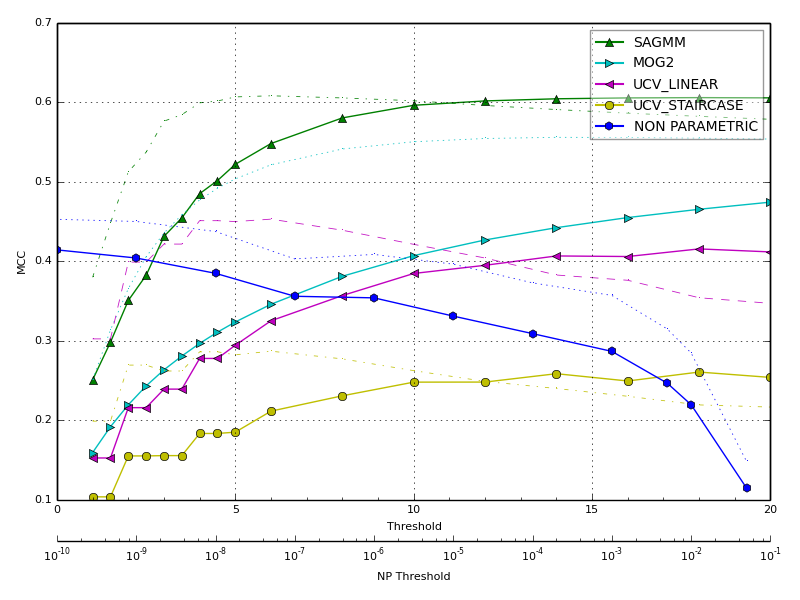
\includegraphics[width=80mm]{img/ch6/MCC-plot9-2}}
%\subfigure[F-Measure ($\alpha=0.001$)]%
%{\label{fig:FMeasure-plot9-1}\includegraphics[width=80mm]{img/ch6/FMeasure-plot9-1}}
%\subfigure[F-Measure - ($\alpha=0.0002$)]%
%{\label{fig:FMeasure-plot9-2}\includegraphics[width=80mm]{img/ch6/FMeasure-plot9-2}}
%\subfigure[D-Score ($\alpha=0.001$)]%
%{\label{fig:DSCORE-plot9-1}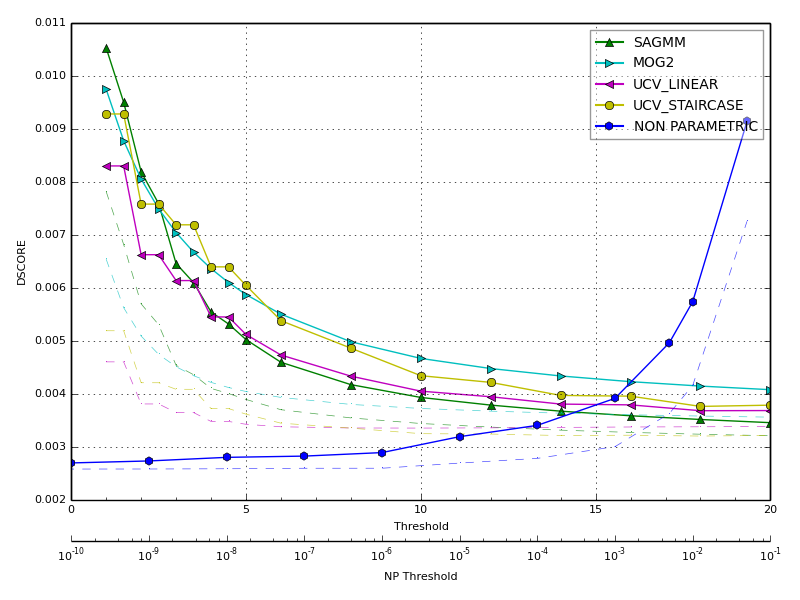
\includegraphics[width=80mm]{img/ch6/DSCORE-plot9-1}}
%\subfigure[D-Score - ($\alpha=0.0002$)]%
%{\label{fig:DSCORE-plot9-2}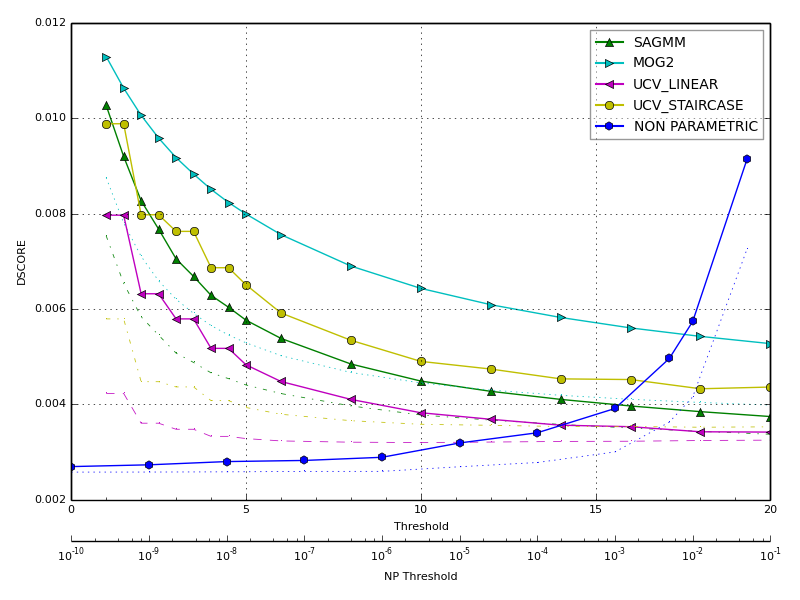
\includegraphics[width=80mm]{img/ch6/DSCORE-plot9-2}}
%\caption[Cuadros comparativos métricas de rendimiento de MCC, F-Measure, y D-Score ($\alpha=0.001$ y $\alpha=0.0002$).]{Cuadros comparativos generales de métricas de rendimiento \textit{MCC}, \textit{F-Measure} y \textit{D-Score} con tasa de aprendizaje $\alpha=0.001$ y $\alpha=0.0002$, lineas segmentadas en los cuadros indican el resultado con morfología}
%\label{fig:pe_metricas_1}
%\end{figure}
%
%
%\begin{figure}[!ht]
%\centering     %%% not \center
%\subfigure[PSNR ($\alpha=0.001$)]%
%{\label{fig:PSNR-plot9-1}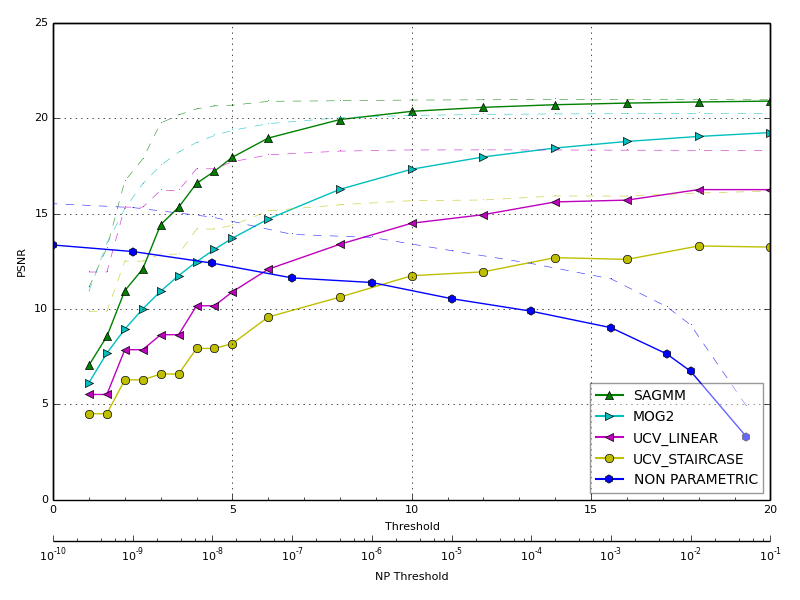
\includegraphics[width=80mm]{img/ch6/PSNR-plot9-1}}
%\subfigure[PSNR - ($\alpha=0.0002$)]%
%{\label{fig:PSNR-plot9-2}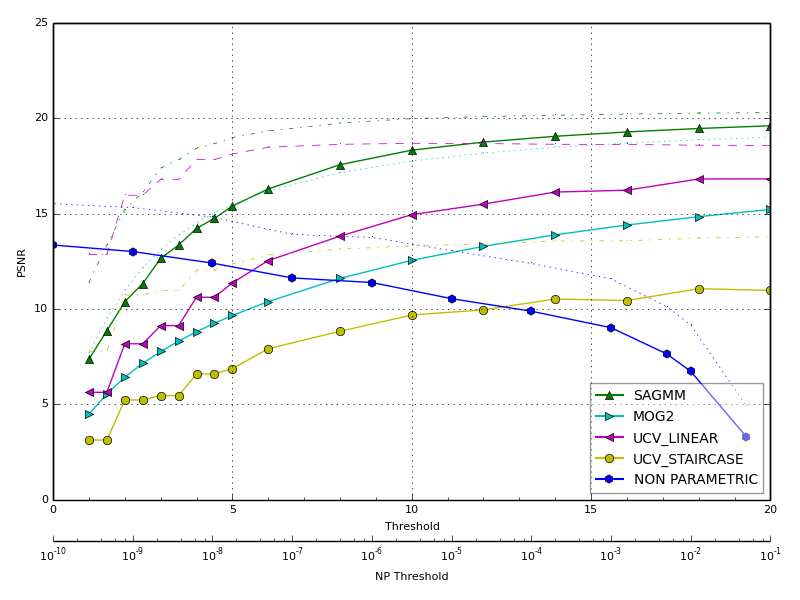
\includegraphics[width=80mm]{img/ch6/PSNR-plot9-2}}
%\subfigure[MSSIM ($\alpha=0.001$)]%
%{\label{fig:MSSIM-plot9-1}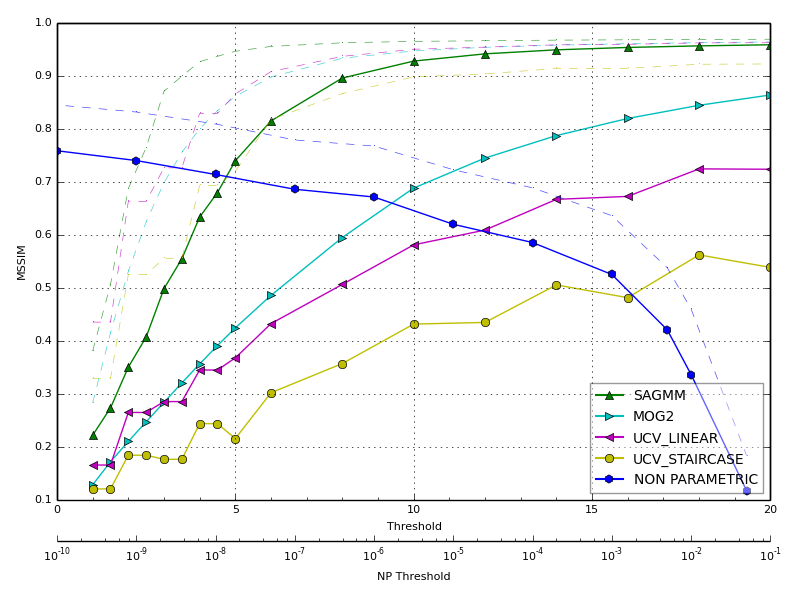
\includegraphics[width=80mm]{img/ch6/MSSIM-plot9-1}}
%\subfigure[MSSIM - ($\alpha=0.0002$)]%
%{\label{fig:MSSIM-plot9-2}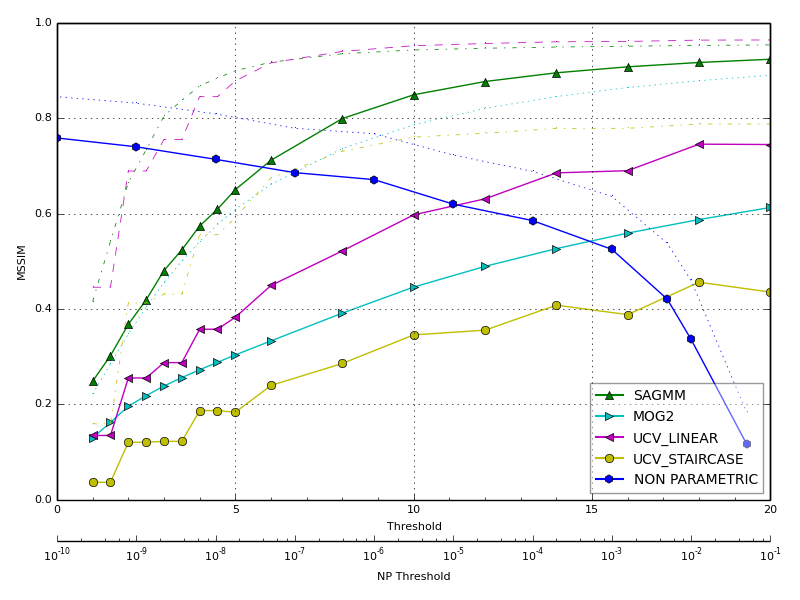
\includegraphics[width=80mm]{img/ch6/MSSIM-plot9-2}}
%\caption[Cuadros comparativos métricas de percepción PSNR y MSSIM ($\alpha=0.001$ y $\alpha=0.0002$).]{Cuadros comparativos generales de métricas de percepción PSNR y MSSIM con las tasas de aprendizaje $\alpha=0.001$ y $\alpha=0.0002$, la líneas segmentadas son los resultados utilizando morfología}
%\label{fig:pe_metricas_2}
%\end{figure}


Los resultados generales de la figuras \ref{fig:pe_metricas_1} y \ref{fig:pe_metricas_2} señalan, desde la perspectiva de las métricas de rendimiento, el valor óptimo de la distancia de \textit{Mahalanobis} que debiera ser elegido para operar con los algoritmo. Sin embargo, estos valores de \textit{threshold} no resultan en mejores puntos en la curva de operaciones características. Esto se evidencia al confrontar las curvas de rendimiento (figuras \ref{fig:pe_metricas_1} y \ref{fig:pe_metricas_2}) con las tablas (\ref{tab:metricas_1}, \ref{tab:metricas_2}, \ref{tab:metricas_3}, y \ref{tab:metricas_4}) de puntos óptimos de operación seleccionados para comparar cada uno de los algoritmos. Por ejemplo, el valor óptimo de \textit{MCC} ($0.61$) y \textit{F-Measure} ($0.60$) en \textit{SAGMM} se alcanza con un \textit{threshold} de $6$ y $10$ ($4.5$ y $5$ con morfología) para $\alpha=0.001$ y $\alpha=0.0002$ respectivamente. Utilizando estos valores óptimos para seleccionar el punto de operación en la curva ROC, resulta en tasas de verdadero y falso positivos inferiores a los escogidos en forma manual, de acuerdo con el criterio del punto más cercano a la zona de clasificación perfecta. El valor $\textit{threshold}=6$ (óptimo de acuerdo con la figura \ref{fig:MCC-plot9-1} de \textit{MCC} para  $\alpha=0.001$) origina el punto $\langle0,62-0,0065\rangle$ en la curva de operaciones, pero el punto de operación seleccionado (tabla \ref{tab:metricas_1}) corresponde al par ordenado $\langle0.76626-0.02246\rangle$, con $\textit{threshold=3.5}$. Esta última selección sacrifica falsos positivos (errores) en 1.6\% (en el rango 0-1), pero mejora el rendimiento de clasificación aumentando la tasa de verdaderos positivos en un 14\%. Contrastando \textit{MCC} ($0.53$) y \textit{F-Measure} ($0.50$) del punto elegido con sus pares del punto óptimo, ambas cifras se diferencian en un 7\% y 10\% respectivamente del punto considerado óptimo. Comparando además el valor de la métrica \textit{D-Score} para ambos puntos en discusión (óptimo y escogido), existe una diferencia de $0.00151$ entre ambas, un 20\% del valor mínimo (notar que para \textit{D-Score} interesa esta métrica sea el mínimo posible), señalando que se ha escogido un punto de operación (no el óptimo) que tolera un 20\% de incremento en errores de bajo costo (pixeles errados que no afectan el reconocimiento de una silueta). El impacto de la diferencia en esta última métrica se puede observar en la figura \ref{fig:sagmm_6} con una menor cantidad de falsos positivos con respecto a la figura \ref{fig:sagmm_3_5}, pero en este último es posible aún reconocer la silueta a pesar de contener más falsos positivos, es decir los falsos positivos no afectarían el proceso de segmentación. En síntesis, la elección del punto de operación es un compromiso que requiere contrastar estas métricas de rendimiento con la curva de operaciones de desempeño del algoritmo para escoger el punto más adecuado con el propósito del algoritmo. Se debe mencionar que el punto de operación es un resultado general, quedan fuera particularidades, y este punto corresponde a un promedio que consolida los distintos resultados del algoritmo enfrentado a las diferentes dificultades que proporcionan las secuencias.

\begin{figure}[!ht]
\centering     %%% not \center
\subfigure[\textit{SAGMM threshold=}$3.5$ ($\alpha=0.001$)]%
{\label{fig:sagmm_3_5}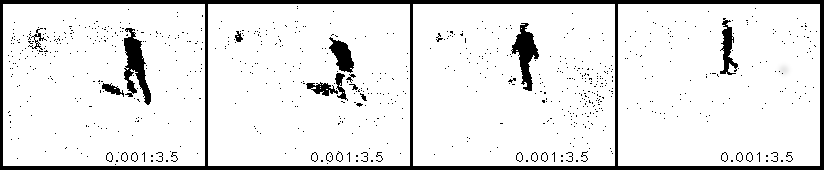
\includegraphics[width=0.75\textwidth]{img/ch6/sagmm_3_5}}
\subfigure[\textit{SAGMM threshold=}$6.0$ ($\alpha=0.001$)]%
{\label{fig:sagmm_6}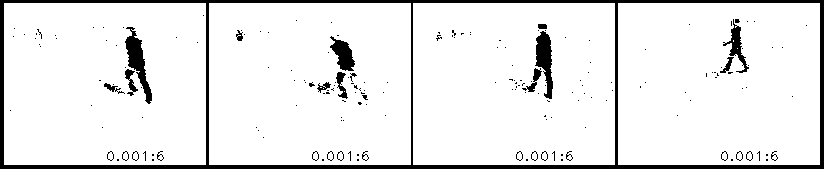
\includegraphics[width=0.75\textwidth]{img/ch6/sagmm_6}}
\caption[Comparación de cuadros con dos distintos valores de \textit{threshold} algoritmo \textit{SAGMM}.]{Comparación de imágenes de diferentes secuencias para dos valores de \textit{threshold} ($3.5$ y $6$) en algoritmo \textit{SAGMM}. Los dos primeros cuadros en ambas filas corresponden a la secuencias con peor desempeño (\textit{RunStop}) y los dos siguientes al mejor desempeño (\textit{WalkTurnBack}).}
\label{fig:frame_sagmm_threshold}
\end{figure}

En promedio, con un factor de aprendizaje en $0.001$ y un \textit{threshold} de $3.5$ (tabla \ref{tab:metricas_1}), el algoritmo SAGMM tiene un rendimiento de un $76.6\%$ en la clasificación de los pixeles de siluetas y un error de $2.2\%$ en la clasificación de pixeles de la imagen de fondo. El algoritmo No-Paramétrico con \textit{threshold} $1x10^{-8}$ tiene una tasa de 80\% en verdaderos positivos, pero un error de 6\% en falsos positivos. En contraste el algoritmo MOG2 tiene un 61\% (\textit{threshold} $6$) tasa de verdaderos positivos y 2.8\% en errores falso positivos,  UCV \textit{Staircase} presenta un 74\% (\textit{threshold} $8$) y un 64\% para UCV \textit{Linear}, ambos con una tasa de falsos negativos similar, cercana al 8.8\%. Los cuadros de la figura \ref{fig:roc_point} confirman lo evidenciado por las curvas de operaciones de la sección anterior, SAGMM tiene un mejor desempeño con respecto a los otros algoritmos. Los valores del coeficiente de correlación MCC (\textit{Matthew’s Correlation Coefficient}) y \textit{F-Measure} aventaja los resultados de los otros algoritmos en todos los casos. En la medida que el valor de MCC se acerca a 1, significa una buena predicción en la clasificación y SAGMM se encuentra en un rango entre $[0.50-0.57]$, siendo su valor máximo $0.6$ ($0.67$ con morfología) . La misma situación ocurre con \textit{F-Measure}, está métrica se entiende como el promedio ponderado de las proporciones \textit{precision} y \textit{recall} y los valores obtenidos durante la experimentación son muy similares al coeficiente de correlación \textit{MCC}. Las figuras \ref{fig:MCC-plot9-1} \ref{fig:MCC-plot9-2}, \ref{fig:FMeasure-plot9-1}, y \ref{fig:FMeasure-plot9-2} revelan que ambas métricas producen similares resultados, las curvas siguen la misma tendencia, por lo que la utilización de estas dos métricas en conjunto no agregan mayor información. El coeficiente de correlación \textit{MCC} es una medida más robusta para predecir el resultado de clasificación, debido que se construye utilizando las 4 mediciones de \textit{TP, FN, TN, y FP} registrados en la matriz de confusión (\ref{fig:confusion_matrix}).  Algo parecido ocurre ocurre con las mediciones de similaridad \textit{PSNR} \cite{signal_zhou_2009} y \textit{MSSIM} \cite{wang_image_2004}, estas métricas intentan evaluar similitud entre dos cuadros, pero en los gráficos \ref{fig:PSNR-plot9-1}, \ref{fig:PSNR-plot9-2}, \ref{fig:MSSIM-plot9-1}, y \ref{fig:MSSIM-plot9-2} se advierte que las curvas tienen el mismo comportamiento, ambas curvas alcanzan un valor cercano al máximo en $threshold=10$, y tienen un incremento lineal entre los valores $1 y 6$ de \textit{threshold}, siendo la pendiente de \textit{MSSIM}, entre estos dos puntos, mayor a la de \textit{PSNR} permitiendo obtener información más detallada ante pequeñas variaciones de \textit{threshold}. Esta característica de similitud entre ambas métricas (para evaluación de siluetas) no aporta mayor información de diferenciación, cualquiera de los dos se puede usar como métrica de evaluación de calidad. Esta semejanza de medición entre ambas métricas se puede explicar por la particularidad de las imágenes que se están evaluando, la medida de similaridad estructural intenta medir calidad simulando el ojo humano. Es muy apropiada para diferenciar distorsiones y ruido en imágenes en escala de grises y colores RGB. Pero en este caso de evaluación de siluetas, se compara sólo imágenes binarias (blanco y negro) y se pierden las particularidades de una imagen como el brillo, contraste que utiliza la métrica \textit{MSSIM} para evaluar calidad de una imagen. Finalmente, a pesar que la medida de \textit{F-Measure} o \textit{MCC} que presenta el algoritmo NP (o las dos versiones de UCV) son menores que \textit{SAGMM}, éste al contrario tiene un mejor valor de \textit{D-Score} (comparativamente menor que los otros algoritmos). Esto indica que NP tiene muchos errores (\textit{F-Measure} bajo por ejemplo), pero esos errores tienen muy bajo costo y no afectarían el reconocimiento de una silueta durante segmentación.





%----------
%As the Mahalanobis distance increases, DTR and FAR decrease
%accordingly. However, a higher DTR and lower FAR are more important. MCC can be used
%to explicitly select the probability tradeoff. The large number is better. A MCC of 1
%represents a perfect prediction. The variation of MCC corresponding to a different threshold
%for MD is given in Figure 4.10(a). It shows that the SAGMM is much better than ZHGMM
%for all thresholds MD  [1, 40], (the increment of MD is 2). The maximum MCC of SAGMM
%is 0.42, but the maximum MCC for ZHGMM is 0.38. Each point of MCC here is the mean of
%each threshold across the entire video (of which only 484 frames include the moving vehicle).
%Obviously, the best cutting point threshold is MD=7. Under the optimal threshold of MD, the
%ROC curve is shown in Figure 4.10(b). The lower rate of FAR is more interesting, for
%instance, FAR<0.021, illustrated by the green dashed vertical line in Figure 4.10(b), the DTR
%of SAGMM is much higher than that of ZHGMM. At the point of FAR = 0.021, the DTR of
%SAGMM is 0.7301, but the DTR of ZHGMM is only 0.5683. The comparison of ACC and

%-------
%Los valores del coeficiente de correlación MCC (\textit{Matthew’s Correlation Coefficient}) y FMeasure para SAGMM son los más altos en las cuatro tablas, esto se interpreta que SAGMM hace una buena predicción de clasificación, y un buen nivel de F-Measure pero el nivel D-Score es el mayor con respecto a los  en las 4 tablas son para SAGMM utilizando los dos factores de aprendizaje, son muy similares en todos los muy similar en todos los casos, En el caso de $\alpha=0.001$ 
%
%
%Los puntos escogidos 
%Las tablas xxx fueron construidas eligiendo el punto de la curva roc mas cercano al punto denominado de clasificación perfecta ($0,1$)
%Se elige el punto más cercano a la zona de clasificación perfecta ($0,1$) como el punto de operación y comparación entre los algoritmos, estos puntos se de un algoritmo. Se elige un punto en la curva de ROC 
%
%
%
%
%
%
%Se puede notar en la tabla \ref{tab:metricas} que la medición de calidad MCC (sección \ref{sub:metricas_percepcion}) es parecida en SAGMM y No-Paramétrico, e inferiores en los demas. Esta métrica de correlación indica , F-Measure es superior en el algoritmo No-Paramétrico  los otros algoritmos .  para TPR y 4.9\% en FPR. En contraste los algoritmo 
%
%clasifica los pixeles de la silueta  , en promedio podría reconocer una silueta términos globales este algoritmo puede reconocer  mayor con respecto a los otros algoritmos, esto significa que este algoritmo en términos globales pa n término de TPR es mayor . ,  el resultado de estos puntos se Para elegir un punto de comparación, se emplean las métricas de calidad PSNR, MCC y las  que emulan percepción (sección \ref{sub:metricas_percepcion}), SSIM (similaridad estructural) , D-Score, para seleccionar un punto de operación que sea un compromiso entre tasa de verdaderos y falsos positivos.  de percgráficas de MSSIM  Las gráficas con las mede MCC, PSNR compara con MOG2 de verdaderos positivos presenta una tasa muy aj de FPR esto se puede interpetrar como se acerca por debajo al algoritmo SAGMM. 



\begin{table}[!ht]
\centering
\scalebox{0.8}{
\begin{tabular}{ l | c  | c | c | c | c}
\hline
Métricas    & SAGMM    & NP          & STAIRCASE & LINEAR & MOG2 \\ \hline  \hline
Threshold & 3.5 & 1e-08 & 8 & 5 & 6 \\ \hline
TPR       & 0.77 & 0.81 & 0.74 & 0.64 & 0.62 \\
FPR       & 0.02 & 0.06 & 0.09 & 0.09 & 0.03 \\ \hline
TPR SE(\%) & 3.73 & 3.24 & 2.50 & 2.33 & 6.27 \\
FPR SE(\%) & 0.35 & 1.14 & 1.21 & 1.80 & 0.97 \\ \hline
MCC & 0.53 & 0.38 & 0.29 & 0.26 & 0.43 \\
FMeasure & 0.51 & 0.32 & 0.22 & 0.21 & 0.42 \\
DSCORE & 6.1e-03 & 2.8e-03 & 4.9e-03 & 5.1e-03 & 5.5e-03 \\
MSSIM & 0.55 & 0.71 & 0.36 & 0.37 & 0.49 \\
PSNR & 15.33 & 12.40 & 10.62 & 10.90 & 14.72 \\ \hline

%Threshold & 3.5 & 1e-08 & 8 & 5 & 6 \\ \hline
%TPR       & 0.766259 & 0.809154 & 0.741512 & 0.644581 & 0.616039 \\
%FPR       & 0.022460 & 0.060560 & 0.088565 & 0.086928 & 0.028779 \\ \hline
%TPR SE(\%) & 3.727385 & 3.235501 & 2.503519 & 2.328320 & 6.268563 \\
%FPR SE(\%) & 0.352403 & 1.138918 & 1.205903 & 1.797249 & 0.973822 \\ \hline
%MCC & 0.530268 & 0.384876 & 0.286282 & 0.259620 & 0.432306 \\
%FMeasure & 0.508079 & 0.323445 & 0.222997 & 0.214049 & 0.416929 \\
%DSCORE & 0.006098 & 0.002798 & 0.004860 & 0.005118 & 0.005501 \\
%MSSIM & 0.554645 & 0.713980 & 0.356990 & 0.367577 & 0.485689 \\
%PSNR & 15.331262 & 12.403333 & 10.623046 & 10.900900 & 14.719836 \\ \hline
\hline
\end{tabular}
}
\caption[Métricas de desempeño con factor de aprendizaje 0.001]{Métricas de desempeño con un factor de aprendizaje 0.001.}
\label{tab:metricas_1}
\end{table}

\begin{table}[!ht]
\centering
\scalebox{0.8}{
\begin{tabular}{ l | c  | c | c | c | c}
\hline
Métricas    & SAGMM    & NP          & STAIRCASE & LINEAR & MOG2 \\ \hline \hline
Threshold & 2.5 & 1e-08 & 4 & 3 & 2 \\ \hline
TPR       & 0.75 & 0.69 & 0.58 & 0.43 & 0.59 \\
FPR       & 0.01 & 0.03 & 0.04 & 0.02 & 0.03 \\ \hline
TPR SE(\%) & 4.01 & 4.25 & 2.30 & 2.61 & 5.99 \\
FPR SE(\%) & 0.43 & 0.83 & 0.81 & 0.64 & 1.20 \\ \hline
MCC & 0.59 & 0.45 & 0.36 & 0.35 & 0.44 \\
FMeasure & 0.57 & 0.42 & 0.34 & 0.35 & 0.43 \\
DSCORE & 5.7e-03 & 2.6e-03 & 3.7e-03 & 3.8e-03 & 5.1e-03 \\
MSSIM & 0.69 & 0.83 & 0.69 & 0.66 & 0.53 \\
PSNR & 16.71 & 15.32 & 14.19 & 15.34 & 15.26 \\

%Threshold & 2.5 & 1e-08 & 4 & 3 & 2 \\ \hline
%TPR       & 0.753518 & 0.693224 & 0.583756 & 0.429919 & 0.592791 \\
%FPR       & 0.013872 & 0.033520 & 0.036542 & 0.018650 & 0.027914 \\ \hline
%TPR SE(\%) & 4.006580 & 4.249748 & 2.299956 & 2.612496 & 5.990657 \\
%FPR SE(\%) & 0.427360 & 0.830465 & 0.813981 & 0.638514 & 1.198226 \\ \hline
%MCC & 0.587427 & 0.450147 & 0.355214 & 0.351503 & 0.442632 \\
%FMeasure & 0.572769 & 0.424576 & 0.337035 & 0.347967 & 0.433774 \\
%DSCORE & 0.005696 & 0.002578 & 0.003719 & 0.003806 & 0.005088 \\
%MSSIM & 0.687463 & 0.831895 & 0.693194 & 0.663054 & 0.530787 \\
%PSNR & 16.713430 & 15.319569 & 14.189528 & 15.340899 & 15.259878 \\ \hline
\hline
\end{tabular}
}
\caption[Métricas de desempeño con factor de aprendizaje 0.001 y morfología]{Métricas de desempeño con un factor de aprendizaje 0.001 y morfología.}
\label{tab:metricas_2}
\end{table}



\begin{table}[!ht]
\centering
\scalebox{0.8}{
\begin{tabular}{ l | c  | c | c | c | c}
\hline
Métricas    & SAGMM    & NP          & STAIRCASE & LINEAR & MOG2 \\ \hline  \hline
Threshold & 5 & 1e-10 & 18 & 10 & 20 \\ \hline
TPR       & 0.76 & 0.78 & 0.61 & 0.58 & 0.67 \\
FPR       & 0.03 & 0.05 & 0.12 & 0.03 & 0.03 \\ \hline
TPR SE(\%) & 3.68 & 3.58 & 3.62 & 2.70 & 3.59 \\
FPR SE(\%) & 0.86 & 1.07 & 3.57 & 0.50 & 1.80 \\ \hline
MCC & 0.52 & 0.41 & 0.26 & 0.38 & 0.47 \\
FMeasure & 0.50 & 0.36 & 0.23 & 0.37 & 0.46 \\
DSCORE & 5.8e-03 & 2.7e-03 & 4.3e-03 & 3.8e-03 & 5.3e-03 \\
MSSIM & 0.65 & 0.76 & 0.46 & 0.60 & 0.61 \\
PSNR & 15.40 & 13.36 & 11.06 & 14.95 & 15.22 \\ \hline


%Threshold & 5 & 1e-10 & 18 & 10 & 20 \\ \hline
%TPR       & 0.757436 & 0.783043 & 0.612697 & 0.576459 & 0.673992 \\
%FPR       & 0.026821 & 0.049066 & 0.119800 & 0.028652 & 0.033884 \\ \hline
%TPR SE(\%) & 3.684577 & 3.581044 & 3.616978 & 2.700730 & 3.586148 \\
%FPR SE(\%) & 0.856569 & 1.071288 & 3.566125 & 0.503087 & 1.804198 \\ \hline 
%MCC & 0.522109 & 0.414371 & 0.260572 & 0.384665 & 0.474487 \\
%FMeasure & 0.499241 & 0.363389 & 0.233142 & 0.370329 & 0.456625 \\
%DSCORE & 0.005764 & 0.002692 & 0.004325 & 0.003822 & 0.005272 \\
%MSSIM & 0.650371 & 0.758782 & 0.456146 & 0.597472 & 0.612927 \\
%PSNR & 15.395948 & 13.355313 & 11.062340 & 14.945326 & 15.222005 \\ \hline
\hline
\end{tabular}
}
\caption[Métricas de desempeño con factor de aprendizaje 0.0002]{Métricas de desempeño con un factor de aprendizaje 0.0002.}
\label{tab:metricas_3}
\end{table}


\begin{table}[!ht]
\centering
\scalebox{0.8}{
\begin{tabular}{ l | c  | c | c | c | c}
\hline
Métricas    & SAGMM    & NP          & STAIRCASE & LINEAR & MOG2 \\ \hline  \hline

Threshold & 3 & 1e-06 & 6 & 2 & 8 \\ \hline
TPR       & 0.73 & 0.72 & 0.52 & 0.51 & 0.65 \\
FPR       & 0.02 & 0.05 & 0.08 & 0.02 & 0.03 \\ \hline
TPR SE(\%) & 3.99 & 3.79 & 2.51 & 3.42 & 3.73 \\
FPR SE(\%) & 0.88 & 1.21 & 2.51 & 1.01 & 2.19 \\ \hline
MCC & 0.58 & 0.41 & 0.29 & 0.40 & 0.54 \\
FMeasure & 0.56 & 0.37 & 0.28 & 0.39 & 0.53 \\
DSCORE & 5.1e-03 & 2.6e-03 & 3.8e-03 & 3.6e-03 & 4.7e-03 \\
MSSIM & 0.80 & 0.77 & 0.67 & 0.69 & 0.74 \\
PSNR & 17.38 & 13.75 & 12.83 & 15.96 & 17.15 \\ \hline


%Threshold & 3 & 1e-06 & 6 & 2 & 8 \\ \hline
%TPR       & 0.725696 & 0.724921 & 0.520514 & 0.507221 & 0.647412 \\
%FPR       & 0.020386 & 0.046377 & 0.079401 & 0.023707 & 0.027123 \\ \hline
%TPR SE(\%) & 3.992106 & 3.793829 & 2.512865 & 3.423359 & 3.728286 \\
%FPR SE(\%) & 0.884614 & 1.213586 & 2.506394 & 1.011908 & 2.193415 \\ \hline
%MCC & 0.576425 & 0.408661 & 0.286846 & 0.398999 & 0.541378 \\
%FMeasure & 0.563756 & 0.368642 & 0.277447 & 0.392837 & 0.534538 \\
%DSCORE & 0.005073 & 0.002592 & 0.003791 & 0.003603 & 0.004668 \\
%MSSIM & 0.804898 & 0.767656 & 0.674732 & 0.689373 & 0.736605 \\
%PSNR & 17.383771 & 13.752657 & 12.833882 & 15.964484 & 17.151703 \\ \hline
\hline
\end{tabular}
}
\caption[Métricas de desempeño con factor de aprendizaje 0.0002 y morfología]{Métricas de desempeño con un factor de aprendizaje 0.0002 y morfología.}
\label{tab:metricas_4}
\end{table}



\begin{figure}[!ht]
\centering     %%% not \center
\subfigure[MCC ($\alpha=0.001$)]%
{\label{fig:MCC-plot9-1}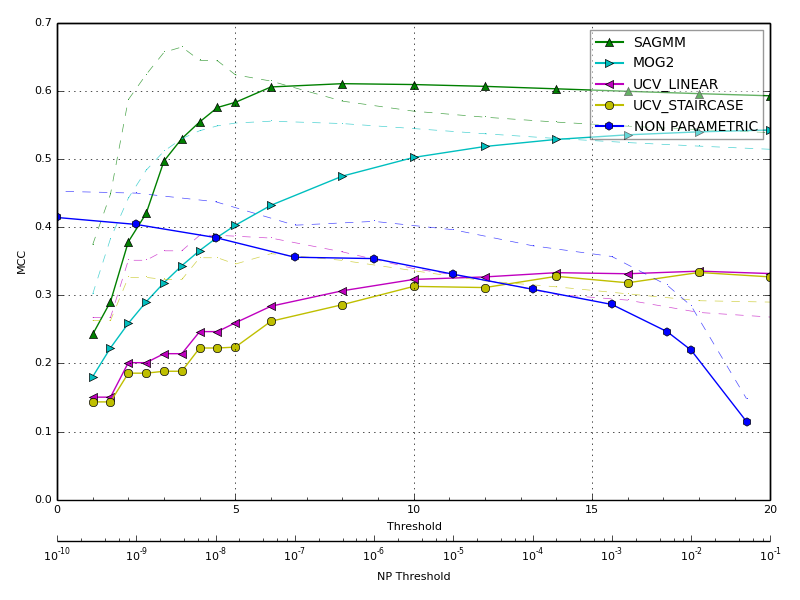
\includegraphics[width=80mm]{img/ch6/MCC-plot9-1}}
\subfigure[MCC ($\alpha=0.0002$)]%
{\label{fig:MCC-plot9-2}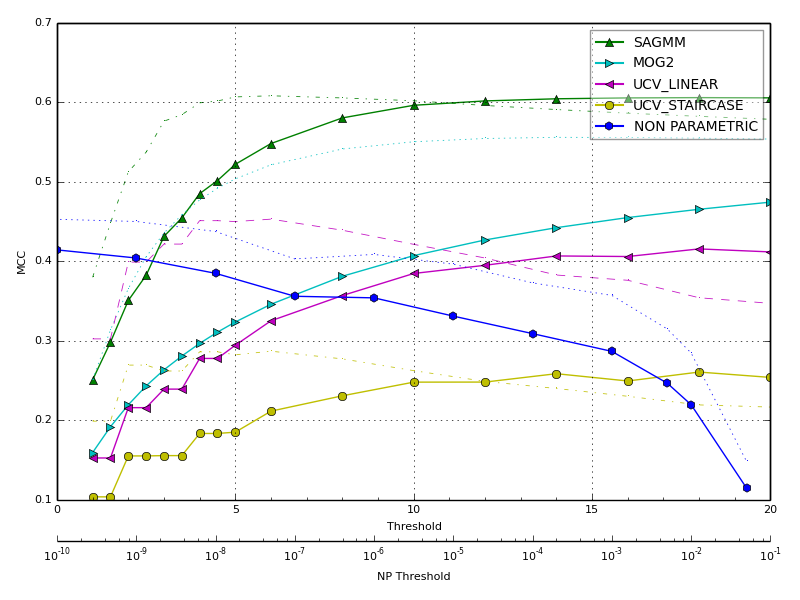
\includegraphics[width=80mm]{img/ch6/MCC-plot9-2}}
\subfigure[F-Measure ($\alpha=0.001$)]%
{\label{fig:FMeasure-plot9-1}\includegraphics[width=80mm]{img/ch6/FMeasure-plot9-1}}
\subfigure[F-Measure - ($\alpha=0.0002$)]%
{\label{fig:FMeasure-plot9-2}\includegraphics[width=80mm]{img/ch6/FMeasure-plot9-2}}
\subfigure[D-Score ($\alpha=0.001$)]%
{\label{fig:DSCORE-plot9-1}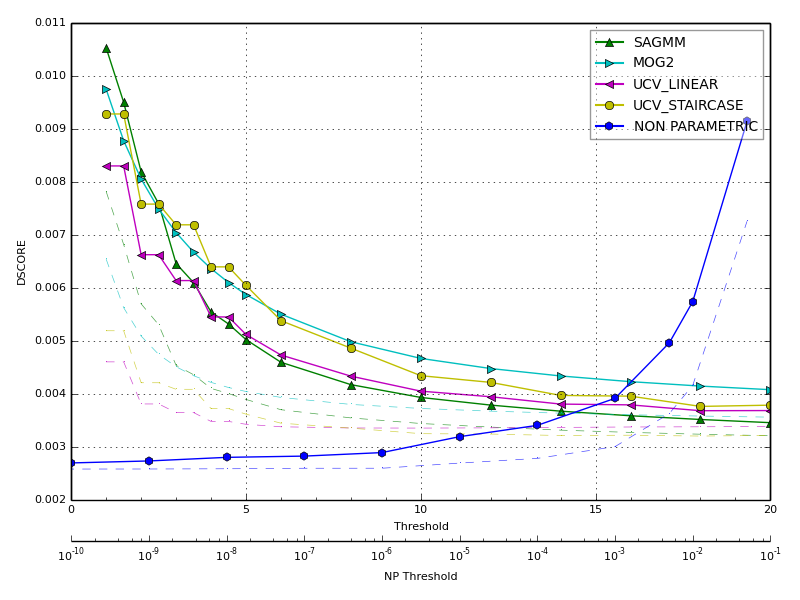
\includegraphics[width=80mm]{img/ch6/DSCORE-plot9-1}}
\subfigure[D-Score - ($\alpha=0.0002$)]%
{\label{fig:DSCORE-plot9-2}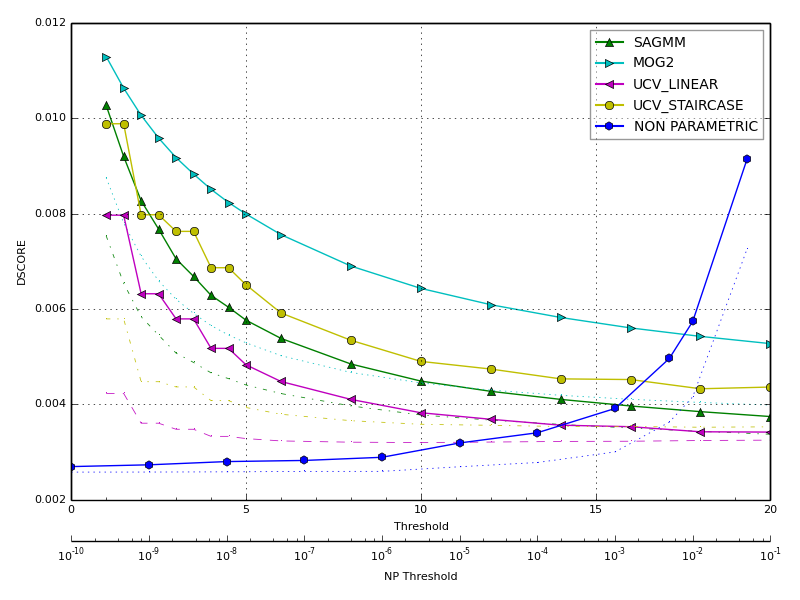
\includegraphics[width=80mm]{img/ch6/DSCORE-plot9-2}}
\caption[Cuadros comparativos métricas de rendimiento de MCC, F-Measure, y D-Score ($\alpha=0.001$ y $\alpha=0.0002$).]{Cuadros comparativos generales de métricas de rendimiento \textit{MCC}, \textit{F-Measure} y \textit{D-Score} con tasa de aprendizaje $\alpha=0.001$ y $\alpha=0.0002$, lineas segmentadas en los cuadros indican el resultado con morfología}
\label{fig:pe_metricas_1}
\end{figure}


\begin{figure}[!ht]
\centering     %%% not \center
\subfigure[PSNR ($\alpha=0.001$)]%
{\label{fig:PSNR-plot9-1}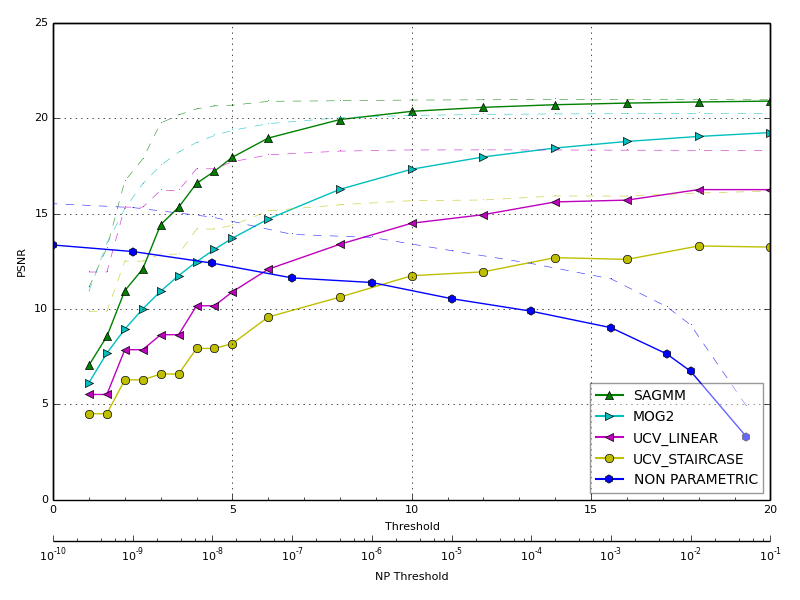
\includegraphics[width=80mm]{img/ch6/PSNR-plot9-1}}
\subfigure[PSNR - ($\alpha=0.0002$)]%
{\label{fig:PSNR-plot9-2}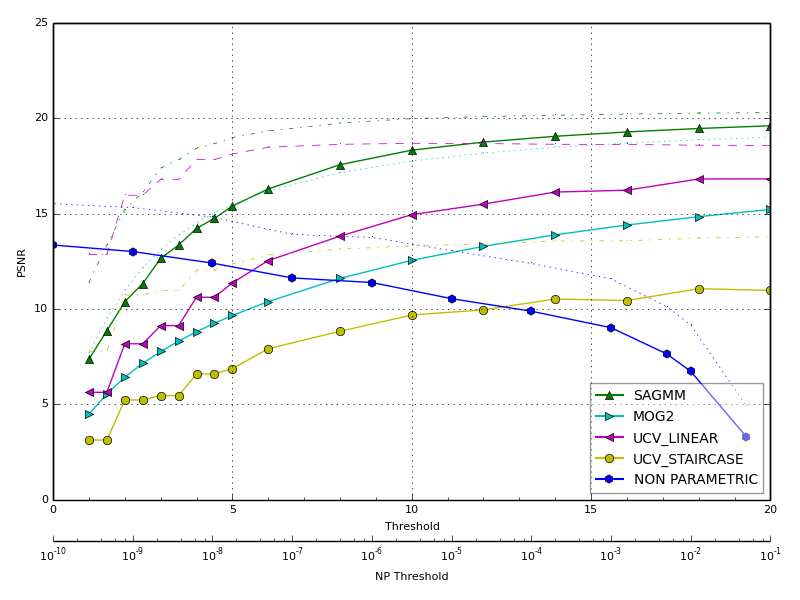
\includegraphics[width=80mm]{img/ch6/PSNR-plot9-2}}
\subfigure[MSSIM ($\alpha=0.001$)]%
{\label{fig:MSSIM-plot9-1}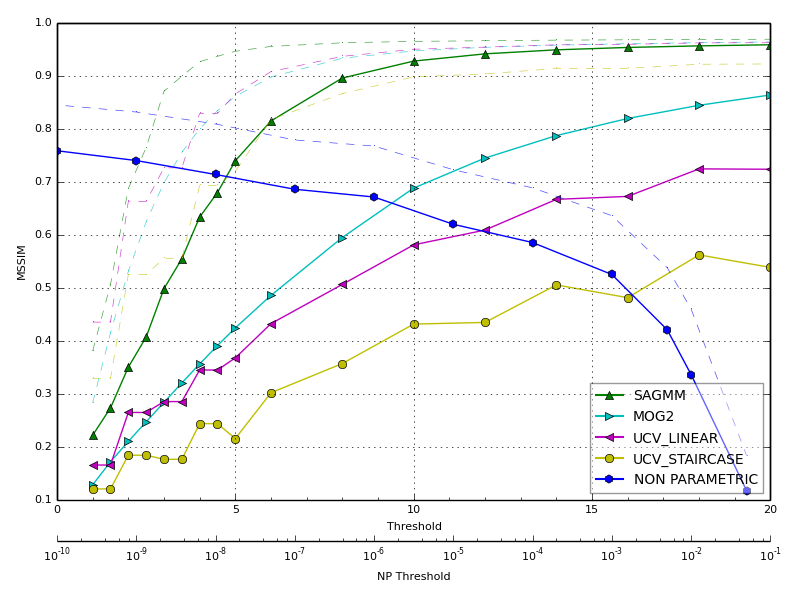
\includegraphics[width=80mm]{img/ch6/MSSIM-plot9-1}}
\subfigure[MSSIM - ($\alpha=0.0002$)]%
{\label{fig:MSSIM-plot9-2}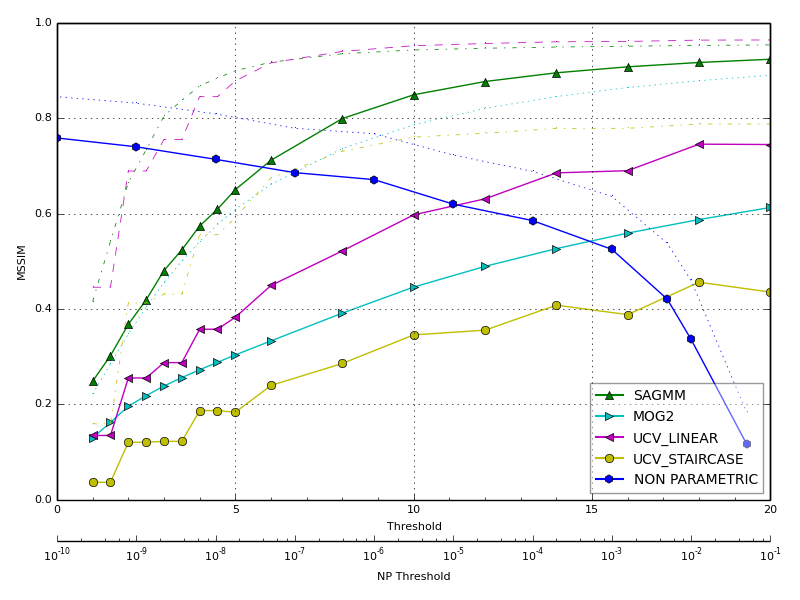
\includegraphics[width=80mm]{img/ch6/MSSIM-plot9-2}}
\caption[Cuadros comparativos métricas de percepción PSNR y MSSIM ($\alpha=0.001$ y $\alpha=0.0002$).]{Cuadros comparativos generales de métricas de percepción PSNR y MSSIM con las tasas de aprendizaje $\alpha=0.001$ y $\alpha=0.0002$, la líneas segmentadas son los resultados utilizando morfología}
\label{fig:pe_metricas_2}
\end{figure}


\begin{figure}[!ht]
\centering     %%% not \center
\subfigure[\textit{SAGMM threshold=}$3.5$ ($\alpha=0.001$)]%
{\label{fig:sagmm_masks}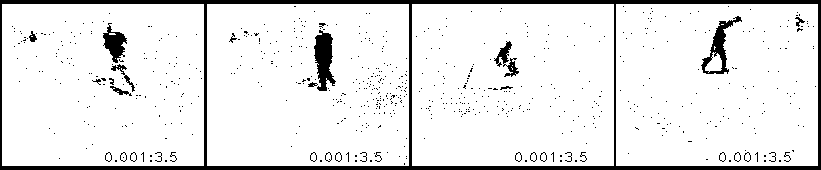
\includegraphics[width=0.75\textwidth]{img/ch6/sagmm_masks}}
\subfigure[\textit{NP threshold=}$1x10^-8$ ($\alpha=0.001$)]%
{\label{fig:np_masks}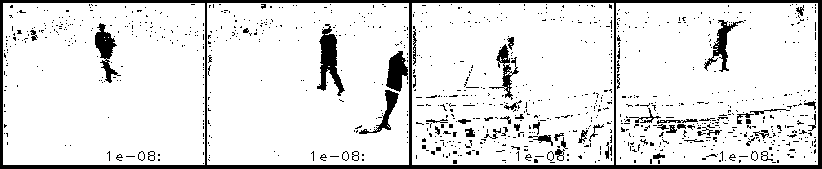
\includegraphics[width=0.75\textwidth]{img/ch6/np_masks}}
\subfigure[\textit{UCV Staircase threshold=}$8$ ($\alpha=0.001$)]%
{\label{fig:ucv_staircase_masks}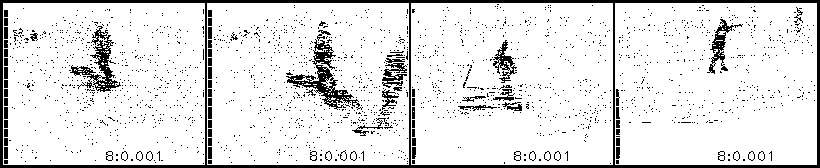
\includegraphics[width=0.75\textwidth]{img/ch6/ucv_staircase_masks}}
\subfigure[\textit{UCV Linear threshold=}$5$ ($\alpha=0.001$)]%
{\label{fig:ucv_linear_masks}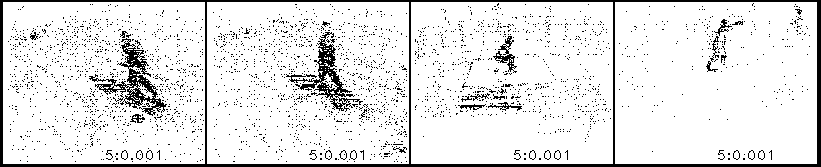
\includegraphics[width=0.75\textwidth]{img/ch6/ucv_linear_masks}}
\subfigure[\textit{MOG2 threshold=}$6$ ($\alpha=0.001$)]%
{\label{fig:mog2_masks}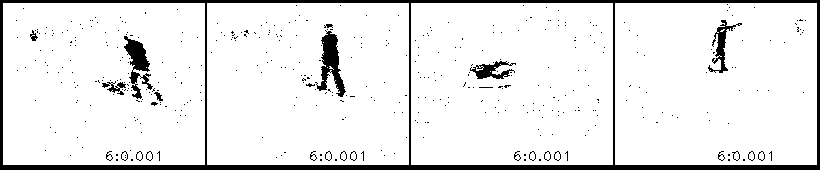
\includegraphics[width=0.75\textwidth]{img/ch6/mog2_masks}}
\caption[Resultado siluetas comparación diferentes algoritmos.]{Imagenes resultantes de los diferentes algoritmos mencionados en la tabla \ref{tab:metricas_1}}
\label{fig:algoritmo_masks}
\end{figure}


\subsection{Intervalo de confianza curva operaciones características}

Las gráficas de la figura \ref{fig:resultado_roc} se construyen realizando un promedio de todas las instancias independientes de experimentación (\textit{Kick Person1 Camera3}, \textit{Kick Person1 Camera4}, \textit{WalkTurnBack Person1 Camera3}, .., etc). La comparación de la respuesta de clasificación entre varios de los algoritmos se complementa con la medición de la varianza de cada punto promediado, y en forma más específica generando intervalos de confianza \cite{confidence_bands_macskassy_2004} alrededor de los puntos TP/FP, que permiten establecer bandas de confianza (probabilidad $1-\alpha=95\%$) alrededor de la curva de operaciones. Existen varias técnicas \cite{fawcett_roc_analysis_2006} para combinar curvas ROC independientes y construir una curva que representa el comportamiento general de todas las instancias involucradas. Una de estas técnicas es `\textit{thresholding averaging}', la cual consiste básicamente en promediar todos los puntos generados por un valor de \textit{threshold} y es el procedimiento mediante el cual se han generado las curvas de la figura \ref{fig:resultado_roc}.  

La figuras \ref{fig:resultado_global_ci_1} y \ref{fig:resultado_global_ci_2} presenta los intervalos de confianza de 95\% de las curvas de operaciones, destacadas en líneas segmentadas azules rodeando la curva promedio. Se agregan además, en líneas segmentadas de otros colores, las curvas promedio por acción destacando el aporte individual a la curva promedio general. Las bandas que envuelven las curvas de operaciones señalan, con una confianza del 95\%, el rango de valores en el cual se encuentra el valor promedio de la tasa de verdaderos positivos, con posibilidad de un 5\% que el valor se encuentre fuera de esta banda. La construcción de estas bandas no toma en cuenta los \textit{FP} (falsos positivos) y usa sólo los intervalos de \textit{TP} (verdadero positivos) para construir las banda de confianza. Los puntos superior e inferior de un intervalo se calculan mediante la ecuación \ref{eq:confidence_interval}, se obtiene el promedio ($\bar{X}_{TP}$) y desviación estándar ($s$) de las muestras generadas de un valor de \textit{threshold}, esto es el valor promedio \textit{TP} de cada secuencia de acción, y finalmente se divide por la raíz cuadrada del número de muestras.

\begin{equation} \label{eq:confidence_interval}
%\bar{X } - 1.96 \ast \frac{s}{\sqrt{n}} \leq \mu_{TPR} \leq \bar{X } + 1.96 \ast \frac{s}{\sqrt{n}} 
\mu \in \bar{X}_{TP} \pm 1.96 \frac{s}{\sqrt{n}} 
\end{equation}

El algoritmo con mayor varianza es \textit{MOG2}, y se manifiesta en la amplitud del ancho de su bandas de confianza comparado con las otras figuras; 6.2\% y 3.5\% ($\alpha=0.001$ y $\alpha=0.0002$ respectivamente) de acuerdo con las tablas \ref{tab:metricas_1} y \ref{tab:metricas_1}. Son las acciones \textit{WalkTurnBack} y \textit{Punch} las que contribuyen con este efecto, debido a la distancia que separa ambas curvas del promedio general. Pero es la acción \textit{Punch} y en menor medida \textit{ShotGunCollapse} las que empeoran el desempeño global, y más específicamente, de acuerdo con la figura \ref{fig:MOG2_Kick} del apéndice \ref{chap:apendice_2}, son las secuencias registradas por la cámara 3 las que deterioran el rendimiento general. Los algoritmos \textit{SAGMM} y \textit{NP} presentan similar intervalos de confianza para los dos factores de aprendizaje, comprobándose en la tabla \ref{tab:metricas_1} con $\alpha=0.001$ \textit{SAGMM} tiene un error estándar (\textit{SE}) de 3.5\% y 3.2\% para el algoritmo \textit{NP}. Con estos valores de confianza se puede afirmar que ambos algoritmos presentan un desempeño similar, porque sus curvas promedios son parecidas, \textit{NP} ligeramente inferior, y sus intervalos de confianza se sobreponen. De esta forma, cualquier punto de las curvas queda delimitado por un 95\% de posibilidad que este dentro de esas bandas. Al igual que \textit{MOG2} son las acciones \textit{Punch} y \textit{ShotGunCollapse} que deterioran el rendimiento en \textit{NP}, pero en este caso son las acciones registradas por la cámara 4 las que disminuyen el desempeño de este algoritmo. Con \textit{SAGMM} son las acciones \textit{RunStop} y menor medida \textit{ShotGunCollapse} que se localizan debajo de la curva de promedio general, con $\alpha=0.0002$ se agrega también \textit{WalkturnBack} especialmente las acciones registradas por la cámara 3, actor \textit{Person4}. A pesar que en términos generales el desempeño de \textit{UCV} en sus dos versiones (\textit{Linear} y \textit{Staircase}) es menor comparado con los otros algoritmos, ambos presentan la menor varianza de todos con $\alpha=0.001$, para $\alpha=0.0002$ se demostró que el desempeño fue notablemente inferior. El error estándar de la tabla \ref{tab:metricas_1} es  de 2.5\% y 2.2\% para   \textit{Staircase} y \textit{Linear} respectivamente, y se verifica además por el menor ancho en los intervalos de confianza en ambas figuras. Todas las curvas de acciones promedio en \textit{Staircase} se encuentran muy ajustadas a su promedio general y en el caso de \textit{Linear} es la acción \textit{ShotGunCollapse} registrada por la cámara 3 y específicamente la acción ejecutada por el actor \textit{Person4}  la que se encuentra debajo del promedio.

La mayoria de la secuencia de acciones registradas por la cámara 3 son las que contribuyen al deterioro del desempeño general, esta cámara particularmente se encuentra en un borde del escenario y la distancia al centro del escenario es mayor de las otra cámara que se encuentra en un costado del escenario. 

%\begin{figure}
%\centering     %%% not \center
%\subfigure[Medida global DScore]
%{\label{fig:DSCORE_SUMMARY_001}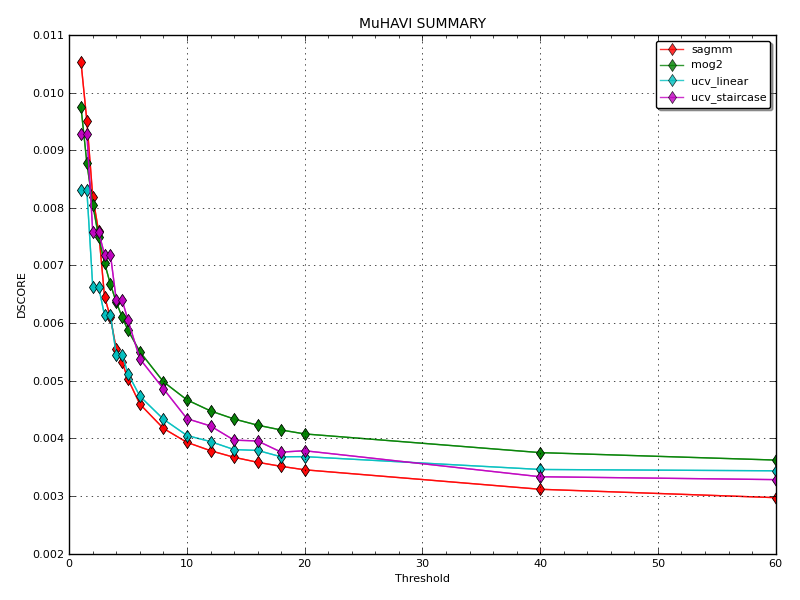
\includegraphics[width=80mm]{img/DSCORE_SUMMARY_001}}
%\subfigure[Medida global de similitud estructural]
%{\label{fig:MSSIM_SUMMARY_001}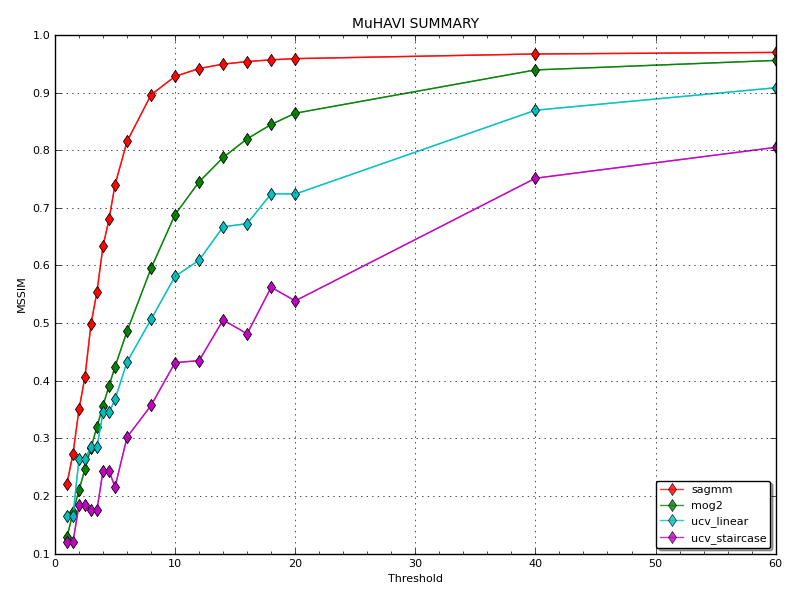
\includegraphics[width=80mm]{img/MSSIM_SUMMARY_001}}
%\subfigure[Coeficiente global de correlation Mathew (MCC)]
%{\label{fig:MCC_SUMMARY_001}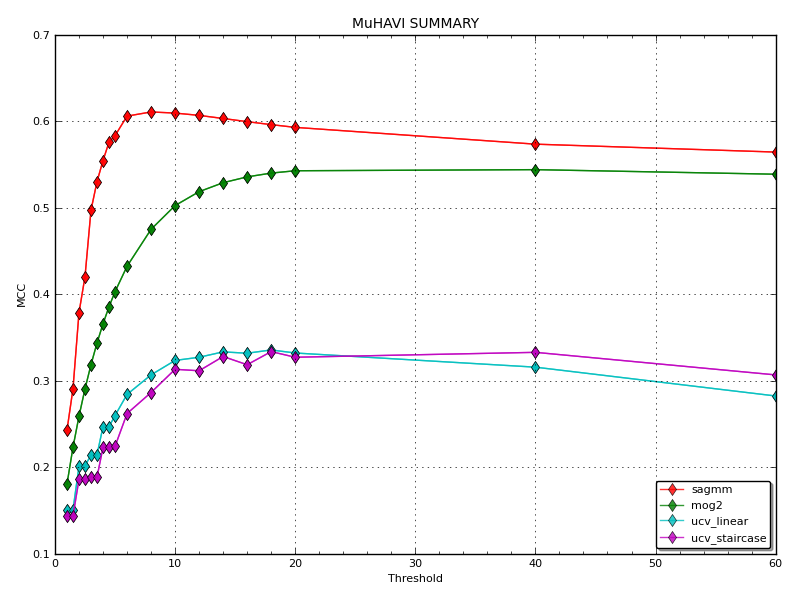
\includegraphics[width=80mm]{img/MCC_SUMMARY_001}}
%\subfigure[Mediciona global de rendimiento obtenido para FMeasure]
%{\label{fig:FMEASURE_001}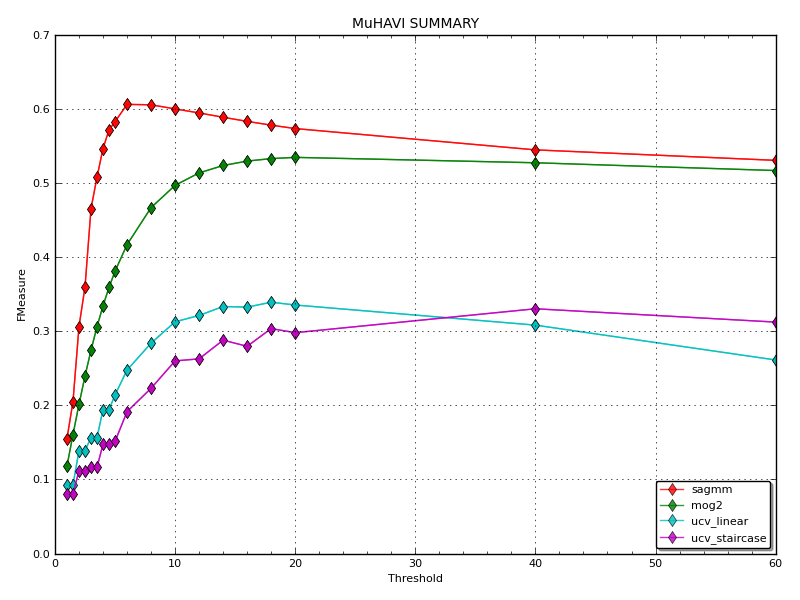
\includegraphics[width=80mm]{img/FMEASURE_001}}
%\subfigure[Medición global de rendimiento PSNR]
%{\label{fig:PSNR_SUMMARY_001}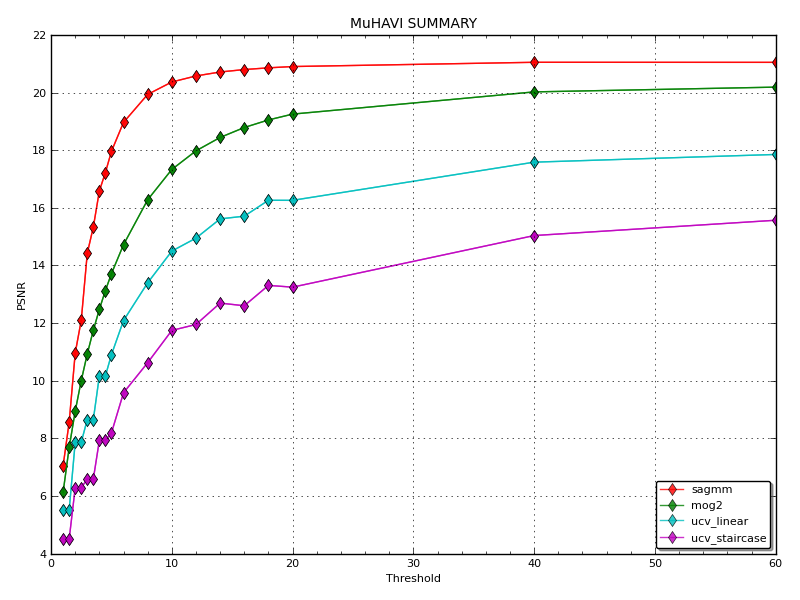
\includegraphics[width=80mm]{img/PSNR_SUMMARY_001}}
%\caption[Mediciones de rendimiento global obtenidos para un factor de aprendizaje $\alpha=0.001$]{Gráficas del rendimiento global de cada algoritmo dejando constante el factor de aprendizaje en $\alpha=0.001$ y modificando el valor de umbral (distancia de Mahalanobis)}
%\label{fig:resultado_global_0.001}
%\end{figure}



\begin{figure}[!ht]
\centering     %%% not \center
\subfigure[SAGMM]
{\label{fig:SAGMM-plot11-1}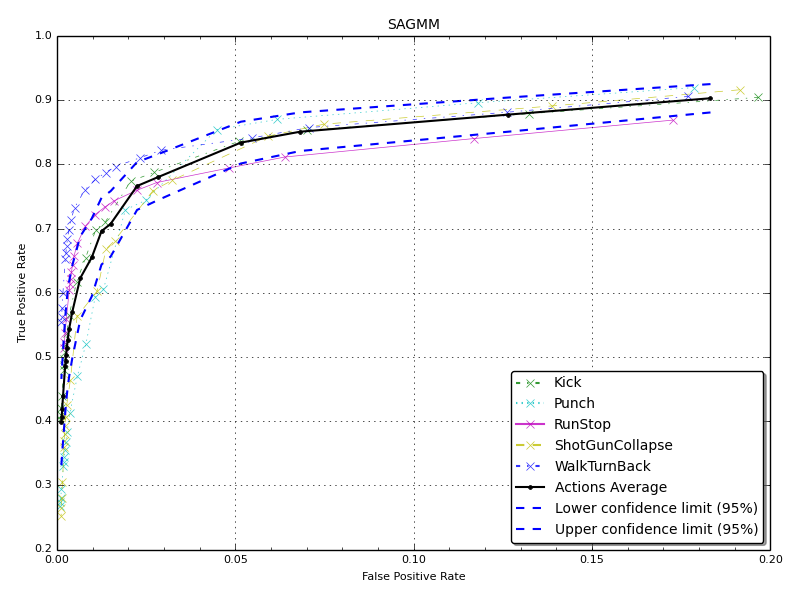
\includegraphics[width=80mm]{img/ch6/SAGMM-plot11-1.png}}
\subfigure[Non Parametric]
{\label{fig:NP-plot11-1}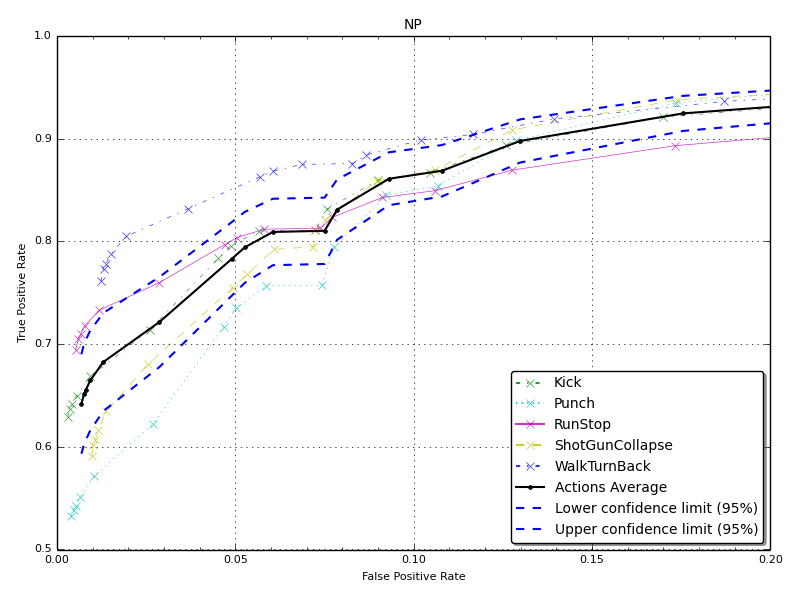
\includegraphics[width=80mm]{img/ch6/NP-plot11-1.png}}
\subfigure[UCV Staircase]
{\label{fig:UCV-STAIRCASE-plot11-1}\includegraphics[width=80mm]{img/ch6/UCV_STAIRCASE-plot11-1.png}}
\subfigure[UCV LINEAR]
{\label{fig:UCV-LINEAR-plot11-1}\includegraphics[width=80mm]{img/ch6/UCV_LINEAR-plot11-1.png}}
\subfigure[MOG2]
{\label{fig:MOG2-plot11-1}\includegraphics[width=80mm]{img/ch6/MOG2-plot11-1.png}}
\caption[Curva operaciones promedio junto con intervalo de confianza de 95\% ($\alpha=0.001$)]{Curvas promedios de operaciones características resultantes separadas por algoritmo con intervalo de confianza de 95\%  ($\alpha=0.001$)}
\label{fig:resultado_global_ci_1}
\end{figure}


\begin{figure}[!ht]
\centering     %%% not \center
\subfigure[SAGMM]
{\label{fig:SAGMM-plot11-2}\includegraphics[width=80mm]{img/ch6/SAGMM-plot11-2.png}}
\subfigure[Non Parametric]
{\label{fig:NP-plot11-2}\includegraphics[width=80mm]{img/ch6/NP-plot11-2.png}}
\subfigure[UCV Staircase]
{\label{fig:UCV-STAIRCASE-plot11-2}\includegraphics[width=80mm]{img/ch6/UCV_STAIRCASE-plot11-2.png}}
\subfigure[UCV LINEAR]
{\label{fig:UCV-LINEAR-plot11-2}\includegraphics[width=80mm]{img/ch6/UCV_LINEAR-plot11-2.png}}
\subfigure[MOG2]
{\label{fig:MOG2-plot11-2}\includegraphics[width=80mm]{img/ch6/MOG2-plot11-2.png}}
\caption[Curva operaciones promedio junto con intervalo de confianza de 95\% ($\alpha=0.0002$)]{Curvas promedios de operaciones características resultantes separadas por algoritmo con intervalo de confianza de 95\%  ($\alpha=0.0002$)}
\label{fig:resultado_global_ci_2}
\end{figure}




%\subsection{Evaluación de acciones}
%Un aspecto adicional es el desafio que presenta MuHAVI como conjunto de datos al ser evaluados con diferentes algoritmosque permiten los resultados experimentales, es poder determinar el grado de dificultad que presenta el conjunto de datos


%\begin{figure}[!ht]
%\centering     %%% not \center
%\subfigure[SAGMM]
%{\label{fig:SAGMM-plot18-1}\includegraphics[width=80mm]{img/ch6/SAGMM-plot18-1.png}}
%\subfigure[Non Parametric]
%{\label{fig:NP-plot18-1}\includegraphics[width=80mm]{img/ch6/NP-plot18-1.png}}
%\subfigure[UCV Staircase]
%{\label{fig:UCV-STAIRCASE-plot18-1}\includegraphics[width=80mm]{img/ch6/UCV_STAIRCASE-plot18-1.png}}
%\subfigure[UCV LINEAR]
%{\label{fig:UCV-LINEAR-plot18-1}\includegraphics[width=80mm]{img/ch6/UCV_LINEAR-plot18-1.png}}
%\subfigure[MOG2]
%{\label{fig:MOG2-plot18-1}\includegraphics[width=80mm]{img/ch6/MOG2-plot18-1.png}}
%\caption[Curva operaciones desagregadas por acción]{Curvas de operaciones desagregadas por acción en cada algoritmo}
%\label{fig:algoritmo_actions_1}
%\end{figure}
%
%\begin{figure}[!ht]
%\centering     %%% not \center
%\subfigure[SAGMM]
%{\label{fig:SAGMM-plot18-2}\includegraphics[width=80mm]{img/ch6/SAGMM-plot18-2.png}}
%\subfigure[Non Parametric]
%{\label{fig:NP-plot18-2}\includegraphics[width=80mm]{img/ch6/NP-plot18-2.png}}
%\subfigure[UCV Staircase]
%{\label{fig:UCV-STAIRCASE-plot18-2}\includegraphics[width=80mm]{img/ch6/UCV_STAIRCASE-plot18-2.png}}
%\subfigure[UCV LINEAR]
%{\label{fig:UCV-LINEAR-plot18-2}\includegraphics[width=80mm]{img/ch6/UCV_LINEAR-plot18-2.png}}
%\subfigure[MOG2]
%{\label{fig:MOG2-plot18-2}\includegraphics[width=80mm]{img/ch6/MOG2-plot18-2.png}}
%\caption[Curva operaciones desagregadas por acción]{Curvas de operaciones desagregadas por acción en cada algoritmo}
%\label{fig:algoritmo_actions_1}
%\end{figure}
%


%\textit{Ghost} : La imagen de fondo cambia principalmente por dos factores, variaciones de las condiciones de iluminación, nubes que ocultan el solo, luz de una habitación que se apagan o encienden. Objetos que modifican su estado detenido a movimiento o viceversa. Detección de fantasma ("ghost") es cuando algún elemento que era parte del fondo comienza a desplazarse, el mecasnimo de eliminación de fondo de los algoritmos, detectaran dos áreas; el área donde el objeta se encuentra actualmente localizado, y la zona donde se encontraba el objeto antes de iniciar el movimiento. Esta última zona se conoce como fantasma, dado que esta no corresponde a ningún objeto en movimiento.
% eliminación de fondo se refiere a elementos que estaban en el fondo y comienzan a moverse. 
% Es cuando objetos que estaban en el fondo comienzan  (nubes que cubren el sol) 


\newpage
\section{Resumen}

En este capítulo se ha enfocado principalmente en describir y analizar los distintos resultados obtenidos durante la experimentación, se ha discutido el impacto de estas métricas en la selección de un punto de operación más óptimo. La curva de operaciones características es la herramienta más importante para comparar desempeño entre distintos algoritmos. Mediante la observación visual es posible discriminar y determinar el mejor desempeño de un algoritmo; sólo localizando la curva cerca del borde superior izquierdo o la que está emplazada sobre las otras. Una forma más precisa de diferenciar consiste en comparar el área bajo la curva que generan las curvas de operaciones, dentro de un rango específico de evaluación. Se ha discutido también, la forma de encontrar un punto de operación óptimo dentro de la curva operaciones, contrastando está selección con las métricas de rendimiento mencionadas en el capítulo~\ref{chap:metricas}. Se ha demostrado que las métricas de \textit{MCC} y \textit{F-Measure} son indicadores de calidad muy parecidos, en la evaluación de desempeño de los algoritmos propuestos para este proyecto, al ser operados sobre el conjunto de datos MuHAVI. Asimismo, \textit{D-Score} resulta una buena métrica para discriminar falsas alarmas (falsos positivos) de poco impacto que no afectan el reconocimiento de imágenes. También se ha notado que las métricas \textit{PSNR} y \textit{MSSIM}, que miden similaridad entre imágenes, tienen una curva de respuesta análoga a las variaciones de \textit{threshold}. La característica principal de la herramienta de similaridad (\textit{MSSIM}) no es apropiada para medir calidad de los resultados, debido que las imágenes que se evalúan pierden las características particulares que contienen las imágenes en escala de grises o colores. En síntesis, las curvas de operaciones, en complemento con las métricas de correlación (\textit{MCC}) y \textit{D-Score} constituyen un buen conjunto de herramientas, que permiten conseguir el punto de operación apropiado,  un compromiso entre una buena discriminación y una buena detección de siluetas.

